% =====================================================================
\section{Results}
\label{sec:results}

All results in \S\ref{sec:res-ensemble} to \S\ref{sec:res-recon} are means over
the rolling windows; \S\ref{sec:res-final} gives the final windows of the first
version.

\subsection{The ensemble is the most accurate item-by-store forecast}
\label{sec:res-ensemble}

\begin{table*}[t]
\centering
\caption{\textbf{Over the rolling windows the equal-weight ensemble has the lowest item-by-store error on
\rcount{enslowestixs} of nine data sets, is in the 90\% model confidence set item by store on \rcount{ensinsetixs}
and at the total on \rcount{ensinsettotal}.} Mean WRMSSE over the rolling
windows (lower is better); W: windows. Bold: the lowest in the row. $^{\circ}$: in the 90\% model confidence set of
the row (Hansen, Lunde and Nason, range statistic, bootstrap over windows; Timestral, added in study F, is not
in the comparison). Ensemble: the equal-weight mean of the world model, LightGBM and TimesFM with the plan,
fixed before any rolling result. Neural models are one fit (seed~1). The Temporal Fusion Transformer was not run on M5
or Favorita, Chronos-Bolt, TimesFM and TFT not on Favorita. Timestral+plan is Timestral-28M with the plan (study F).}
\label{tab:rolling}
\footnotesize
\setlength{\tabcolsep}{3.4pt}
\begin{tabular}{lc*{10}{r}}
\toprule
\textbf{Data} & \textbf{W} & \rotatebox{70}{Ensemble} & \rotatebox{70}{World model} & \rotatebox{70}{Lift model} & \rotatebox{70}{LightGBM} & \rotatebox{70}{TimesFM+plan} & \rotatebox{70}{TimesFM} & \rotatebox{70}{Chronos-Bolt} & \rotatebox{70}{TFT} & \rotatebox{70}{Timestral+plan} & \rotatebox{70}{Seas.\ naive} \\
\midrule
\addlinespace[2pt]\multicolumn{12}{l}{\itshape Item by store} \\
Cheese & 6 & 0.934 & 1.713 & 1.119 & \textbf{0.623}$^{\circ}$ & 0.659 & 0.749 & 0.762 & 0.696 & 1.956 & 1.117 \\
Snack crackers & 6 & \textbf{0.562}$^{\circ}$ & 0.595 & 0.598 & 0.578 & 0.605 & 0.677 & 0.708 & 0.654 & 1.944 & 1.010 \\
Soft drinks & 6 & \textbf{0.536}$^{\circ}$ & 0.600 & 0.672 & 0.545$^{\circ}$ & 0.609 & 0.711 & 0.720 & 0.640 & 0.872 & 0.960 \\
Bottled juice & 6 & \textbf{0.585}$^{\circ}$ & 0.656 & 0.616 & 0.605 & 0.636 & 0.712 & 0.728 & 0.676 & 1.459 & 1.079 \\
Analgesics & 6 & 0.650$^{\circ}$ & 0.672 & 0.677 & \textbf{0.647}$^{\circ}$ & 0.679 & 0.734 & 0.745 & 0.693 & 2.111 & 0.997 \\
Frozen entrees & 6 & \textbf{0.408}$^{\circ}$ & 0.433 & 0.449 & 0.410$^{\circ}$ & 0.487 & 0.549 & 0.554 & 0.488 & 1.048 & 0.710 \\
Frat & 4 & \textbf{0.549}$^{\circ}$ & 0.595 & 0.590 & 0.570 & 0.578 & 0.775 & 0.778 & 0.652 & 0.864 & 1.077 \\
M5 & 4 & \textbf{0.834}$^{\circ}$ & 0.851 & 0.845 & 0.861 & 0.842 & 0.842 & 0.858 & -- & 0.894 & 1.163 \\
Favorita & 4 & \textbf{0.694}$^{\circ}$ & 0.726 & 0.744 & 0.719 & 0.712 & -- & -- & -- & 0.731 & 0.992 \\
\addlinespace[2pt]\multicolumn{12}{l}{\itshape Total} \\
Cheese & 6 & \textbf{0.371}$^{\circ}$ & 0.585$^{\circ}$ & 0.617$^{\circ}$ & 0.456$^{\circ}$ & 0.584 & 0.718 & 0.790 & 0.481$^{\circ}$ & 4.606 & 1.175 \\
Snack crackers & 6 & 1.181$^{\circ}$ & 1.454$^{\circ}$ & \textbf{1.026}$^{\circ}$ & 1.097$^{\circ}$ & 1.181$^{\circ}$ & 1.581$^{\circ}$ & 4.410$^{\circ}$ & 1.301$^{\circ}$ & 16.272 & 1.790$^{\circ}$ \\
Soft drinks & 6 & 0.834$^{\circ}$ & 0.879$^{\circ}$ & 0.965$^{\circ}$ & \textbf{0.831}$^{\circ}$ & 0.977 & 1.157 & 1.270 & 0.971 & 4.181 & 1.035 \\
Bottled juice & 6 & \textbf{0.525}$^{\circ}$ & 0.613$^{\circ}$ & 0.585$^{\circ}$ & 0.530$^{\circ}$ & 0.766$^{\circ}$ & 0.898 & 0.897 & 0.793 & 6.257 & 1.390 \\
Analgesics & 6 & \textbf{0.782}$^{\circ}$ & 0.826$^{\circ}$ & 0.868$^{\circ}$ & 0.869$^{\circ}$ & 0.848$^{\circ}$ & 0.900$^{\circ}$ & 0.979 & 1.057$^{\circ}$ & 31.256 & 1.796 \\
Frozen entrees & 6 & 0.342$^{\circ}$ & 0.338$^{\circ}$ & 0.387$^{\circ}$ & \textbf{0.321}$^{\circ}$ & 0.481 & 0.500 & 0.578 & 0.380 & 2.158 & 0.620 \\
Frat & 4 & 0.337$^{\circ}$ & 0.457 & 0.405$^{\circ}$ & 0.360$^{\circ}$ & \textbf{0.327}$^{\circ}$ & 0.541 & 0.605 & 0.425 & 1.048 & 0.964 \\
M5 & 4 & 0.706$^{\circ}$ & \textbf{0.609}$^{\circ}$ & 1.163$^{\circ}$ & 0.693$^{\circ}$ & 1.035 & 1.000 & 1.333 & -- & 1.025 & 1.087 \\
Favorita & 4 & \textbf{0.303}$^{\circ}$ & 0.341$^{\circ}$ & 0.452 & 0.309$^{\circ}$ & 0.397 & -- & -- & -- & 0.403 & 0.501 \\
\bottomrule
\end{tabular}
\end{table*}


\begin{figure*}[t]
\centering
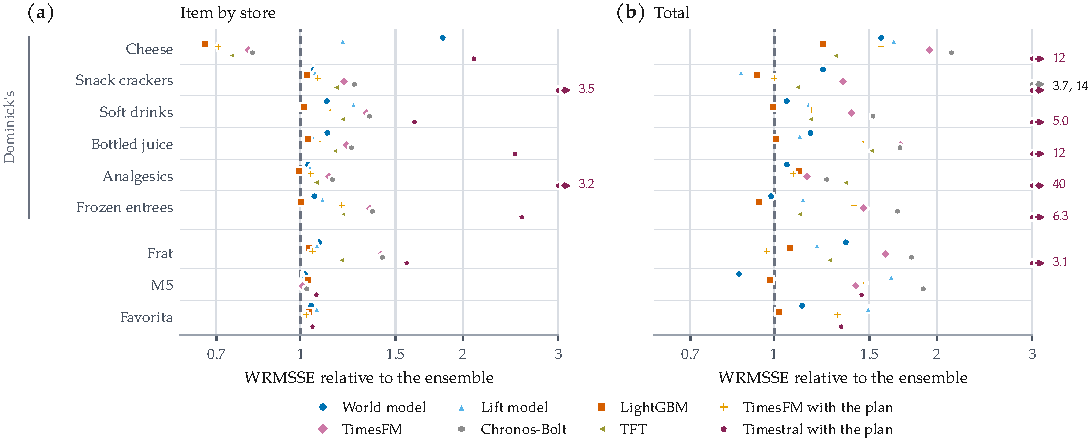
\includegraphics[width=\textwidth]{figs/fig_rolling.pdf}
\caption{\textbf{Item by store, every single model is less accurate than the
ensemble on almost every data set; at the total the ensemble is never far from
the best and the best single model changes with the data set.} Mean WRMSSE over
the rolling windows of each model divided by the ensemble's (dashed line at 1;
log scale; left of the line is more accurate than the ensemble).
\textbf{(a)} Item by store. \textbf{(b)} Chain total. Values beyond the axis are
marked at its edge with their value. Six, four, four and four windows on
Dominick's, Frat, M5 and Favorita.}
\label{fig:rolling}
\end{figure*}

The equal-weight ensemble has the lowest item-by-store error on
\rcount{enslowestixs} of the nine data sets (Table~\ref{tab:rolling},
Figure~\ref{fig:rolling}a). In the other two, analgesics and cheese, LightGBM
is lower: \rv{ana}{lgb}{ixs} against \rv{ana}{ens}{ixs} in analgesics, where
both are in the model confidence set, and \rv{che}{lgb}{ixs} against
\rv{che}{ens}{ixs} in cheese, the one data set where LightGBM is alone in the
set. The ensemble is in the 90\% model confidence set item by store on
\rcount{ensinsetixs} data sets and alone in it on
\rcount{ensaloneixs} (\rcount{ensaloneixslist}). At the chain total it is in
the set on all \rcount{ensinsettotal}, and it has the lowest error on
\rcount{enslowesttotal}; elsewhere the lowest belongs to
\rcount{lowesttotallist}.

By the paired test over windows, the ensemble is more accurate than LightGBM
item by store on \rcount{ensbeatslgbixs} of the eight data sets with paired
results (\rcount{ensbeatslgbixslist}; M5: \rv{mfive}{ens}{ixs} against
\rv{mfive}{lgb}{ixs}) and at the total on \rcount{ensbeatslgbtotal}
(\rcount{ensbeatslgbtotallist}). It is more accurate than the world model item
by store on \rcount{ensbeatsworldixs} and at the total on
\rcount{ensbeatsworldtotal} (\rcount{ensbeatsworldtotallist}). It is less
accurate than either at either level on none. The Temporal Fusion Transformer,
Chronos-Bolt and TimesFM from history alone are behind the ensemble item by store
on every data set where they ran.

The cheese result comes from one window. In one of the six cheese windows the
world model's item-by-store WRMSSE was \rwin{che}{world}{ixsmax}, against a
median of \rwin{che}{world}{ixsmedian} over the six, and the lift model's
\rwin{che}{lift}{ixsmax}; the ensemble, a third of whose forecast is the world
model's, inherits part of that error.

\subsection{What the world model adds to the ensemble}
\label{sec:res-adds}

\begin{table*}[t]
\centering
\caption{\textbf{Removing the world model makes the ensemble less accurate item by store on \rcount{withoutworldmodelixsens}
data sets and at the total on \rcount{withoutworldmodeltotalens}; replacing it with the lift model, the same network
without the carried state, does so on \rcount{liftforworldmodelixsens} and \rcount{liftforworldmodeltotalens}.}
Mean WRMSSE of each variant minus the ensemble's over the rolling windows (study A, added after the rolling results);
above zero the ensemble is more accurate. Bold: the ensemble is more accurate and the 95\% interval from the bootstrap
over windows excludes zero; underlined: the variant is, with the same test. No X: the equal-weight mean of the other two
members ($-$World: without the world model; $-$LGB: without LightGBM; $-$TFM+p: without TimesFM with the plan). Lift:
the world model replaced by the lift model. Fitted: weights chosen on the earlier
windows of the data set (lowest mean WRMSSE over all levels), scored on the next, so one window fewer.}
\label{tab:ablation}
\footnotesize
\setlength{\tabcolsep}{3.2pt}
\begin{tabular}{l*{10}{r}}
\toprule
 & \multicolumn{5}{c}{\textbf{Item by store}} & \multicolumn{5}{c}{\textbf{Total}} \\
\cmidrule(lr){2-6}\cmidrule(lr){7-11}
\textbf{Data} & $-$World & $-$LGB & $-$TFM+p & Lift & Fitted & $-$World & $-$LGB & $-$TFM+p & Lift & Fitted \\
\midrule
Cheese & \textminus 0.328 & \textbf{0.199} & \textbf{0.190} & \textminus 0.196 & \textbf{0.015} & 0.072 & \textbf{0.056} & 0.029 & 0.021 & 0.056 \\
Snack crackers & 0.002 & \textbf{0.018} & 0.004 & 0.002 & 0.004 & \textminus 0.095 & 0.118 & 0.013 & \textminus 0.145 & \textminus 0.073 \\
Soft drinks & 0.008 & \textbf{0.023} & 0.009 & \textbf{0.015} & \textminus 0.006 & 0.025 & \textbf{0.045} & \textminus 0.022 & \textminus 0.007 & \textminus 0.008 \\
Bottled juice & \textbf{0.012} & \textbf{0.016} & \textbf{0.015} & 0.002 & 0.000 & \textbf{0.103} & 0.031 & \textminus 0.042 & 0.051 & \textminus 0.015 \\
Analgesics & 0.000 & \textbf{0.014} & \textminus 0.001 & \textbf{0.003} & \textbf{0.008} & 0.019 & \textminus 0.006 & 0.038 & \textbf{0.025} & 0.012 \\
Frozen entrees & \textbf{0.012} & \textbf{0.019} & \textminus 0.002 & 0.005 & \textminus 0.001 & \textbf{0.025} & \textbf{0.034} & \textminus 0.026 & 0.013 & \textminus 0.015 \\
Frat & 0.002 & \textbf{0.010} & \textbf{0.012} & 0.001 & \textbf{0.007} & \underline{\textminus 0.040} & \textbf{0.021} & \textbf{0.051} & \textminus 0.017 & \underline{\textminus 0.022} \\
M5 & \textbf{0.005} & 0.003 & \textbf{0.006} & \textminus 0.001 & \textbf{0.013} & \textbf{0.113} & 0.050 & \underline{\textminus 0.112} & 0.000 & \textminus 0.037 \\
Favorita & \textbf{0.007} & \textbf{0.006} & \textbf{0.007} & \textbf{0.010} & \textbf{0.007} & 0.037 & 0.013 & \underline{\textminus 0.015} & \textbf{0.067} & 0.004 \\
\bottomrule
\end{tabular}
\end{table*}


\begin{figure*}[t]
\centering
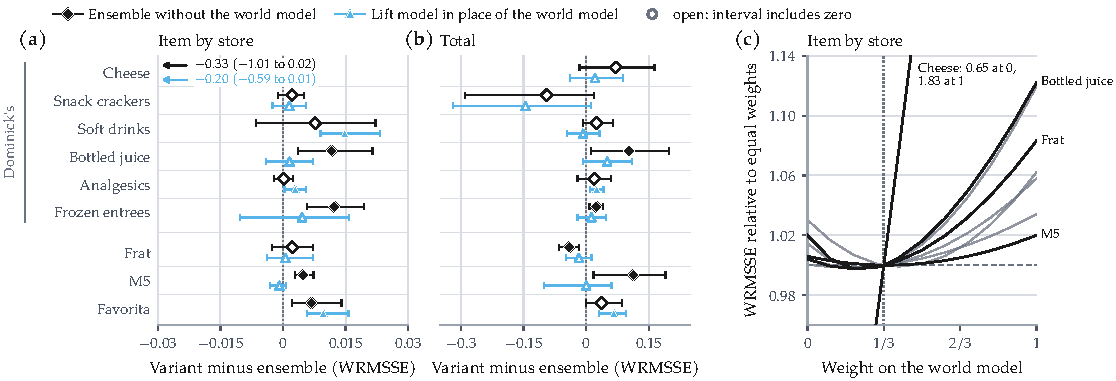
\includegraphics[width=\textwidth]{figs/fig_ablation.pdf}
\caption{\textbf{Taking the world model out of the ensemble costs accuracy on
some data sets; replacing it with the same network without the carried state
costs less often.} \textbf{(a, b)} Mean WRMSSE of the ensemble without the
world model, and with the lift model in its place, minus the ensemble's, with
95\% intervals from the bootstrap over windows; right of zero the ensemble with
the world model is more accurate; filled markers: the interval excludes zero.
\textbf{(a)} Item by store. \textbf{(b)} Total. \textbf{(c)} Item by store:
the ensemble's WRMSSE as the world model's weight goes from 0 to 1 (the other
two sharing the rest equally), relative to equal weights (dotted line at
one third), one line per data set. Study A, saved forecasts only.}
\label{fig:ablation}
\end{figure*}

Each member earns its place on some data sets and none on all
(Table~\ref{tab:ablation}). Without the world model the ensemble is less
accurate item by store on \rcount{withoutworldmodelixsens}
(\rcount{withoutworldmodelixsenslist}) and at the total on
\rcount{withoutworldmodeltotalens} (\rcount{withoutworldmodeltotalenslist}); on
Frat at the total it is more accurate without it
(\rab{frat}{withoutworldmodel}{total}{meandiff}). Without LightGBM it is less
accurate item by store on \rcount{withoutlightgbmixsens} and at the total on
\rcount{withoutlightgbmtotalens}. Without TimesFM with the plan it is less
accurate item by store on \rcount{withouttimesfmixsens}, at the total on
\rcount{withouttimesfmtotalens}, and more accurate at the total on
\rcount{withouttimesfmtotalvar} (\rcount{withouttimesfmtotalvarlist}).
LightGBM is the member the ensemble can least do without.

Some of the world model's contribution is any third model's. With the lift
model in its place, which has the same encoder, readout, inputs and training and
no carried state, the ensemble is less accurate item by store on
\rcount{liftforworldmodelixsens} data sets (\rcount{liftforworldmodelixsenslist})
and at the total on \rcount{liftforworldmodeltotalens}
(\rcount{liftforworldmodeltotalenslist}), and more accurate on none. The carried
state therefore adds to the ensemble where those intervals exclude zero, and
elsewhere the gain from the world model is a gain from adding a third,
different model.

Equal weights are hard to beat. Weights chosen on the earlier windows of each
data set, for item by store, for the total or for all levels, and scored on the
next window, are more accurate than equal weights in \rcount{fittedwins} of
\rcount{fittedn} comparisons and less accurate in \rcount{fittedlosses}. The
fitted weights do say where each member is useful: chosen for the total, the
world model's mean weight is \rw{ana}{total}{world} in analgesics and
\rw{mfive}{total}{world} on M5, against \rw{ana}{bottom}{world} and
\rw{mfive}{bottom}{world} chosen for item by store. Figure~\ref{fig:ablation}c
shows the item-by-store error is flat across a wide range of the world model's
weight on most data sets, which is why fitting the weights gains little.

\subsection{The world model on its own}
\label{sec:res-world}

On its own the world model is behind LightGBM item by store and level with it
at the total. By the paired test LightGBM is more accurate item by store on
\rcount{lgbbeatsworldixs} of eight data sets (\rcount{lgbbeatsworldixslist})
and at the total on \rcount{lgbbeatsworldtotal} (\rcount{lgbbeatsworldtotallist});
the world model is more accurate than LightGBM on \rcount{worldbeatslgbixs} at
either level. Its lowest error is at the M5 chain total,
\rv{mfive}{world}{total} against \rv{mfive}{lgb}{total} for LightGBM and
\rv{mfive}{ens}{total} for the ensemble, but the windows differ enough that
the difference is not outside its interval (LightGBM minus the world model
\rpair{mfive}{lgb}{world}{total}{meandiff}, interval
\rpair{mfive}{lgb}{world}{total}{lo} to \rpair{mfive}{lgb}{world}{total}{hi}).

Against the lift model, which differs only in the carried state, the world model
is more accurate item by store on \rcount{worldbeatsliftixs}
(\rcount{worldbeatsliftixslist}), less accurate on \rcount{liftbeatsworldixs}
(\rcount{liftbeatsworldixslist}), and level at the total on all eight. Taken
alone, carrying the state forward neither helps nor hurts accuracy in most data
sets. Its value shows in what it adds to the ensemble (\S\ref{sec:res-adds}) and
in category plans (\S\ref{sec:res-decisions}), where the world model has the
lowest cost on \rcount{decworldcat} of eight data sets.

\subsection{How the models use the plan}
\label{sec:res-plan}

\begin{table*}[t]
\centering
\caption{\textbf{All three trained models use the plan. On the weekly data price carries most of it; on M5 the world
model relies on event and SNAP days more than LightGBM does.} Input occlusion on the saved models (study B): one plan input is set to
``nothing planned'' (regular price, lever off) in the forecast periods and the forecast recomputed, with no refitting.
Change in WRMSSE item by store and at the total, in percent (above zero: the forecast gets worse without the input),
and the change in forecast units, in percent, in the periods where the input was on. Mean over the rolling windows (LightGBM on M5: the
last two).}
\label{tab:perturbation}
\footnotesize
\setlength{\tabcolsep}{3.6pt}
\begin{tabular}{l*{9}{r}}
\toprule
 & \multicolumn{3}{c}{\textbf{Item by store (\%)}} & \multicolumn{3}{c}{\textbf{Total (\%)}}
 & \multicolumn{3}{c}{\textbf{Units where on (\%)}} \\
\cmidrule(lr){2-4}\cmidrule(lr){5-7}\cmidrule(lr){8-10}
\textbf{Input occluded} & World & Lift & LGB & World & Lift & LGB & World & Lift & LGB \\
\midrule
\addlinespace[2pt]\multicolumn{10}{l}{\itshape Dominick's} \\
Whole plan & 15 & 13 & 26 & 116 & 97 & 149 & \textminus{}59 & \textminus{}58 & \textminus{}58 \\
Price & 8 & 6 & 20 & 75 & 59 & 115 & \textminus{}45 & \textminus{}41 & \textminus{}49 \\
Promotion & 4 & 2 & 3 & 41 & 38 & 34 & \textminus{}34 & \textminus{}40 & \textminus{}26 \\
\addlinespace[2pt]\multicolumn{10}{l}{\itshape Frat} \\
Whole plan & 36 & 36 & 40 & 229 & 268 & 262 & \textminus{}49 & \textminus{}47 & \textminus{}46 \\
Price & 17 & 16 & 18 & 126 & 152 & 138 & \textminus{}38 & \textminus{}36 & \textminus{}34 \\
Promotion & \textminus{}1 & 6 & 4 & 20 & 99 & 34 & \textminus{}16 & \textminus{}30 & \textminus{}18 \\
Feature & 1 & 2 & 4 & 7 & 23 & 16 & \textminus{}28 & \textminus{}28 & \textminus{}29 \\
Display & 0 & 0 & 2 & 4 & 9 & 4 & \textminus{}18 & \textminus{}19 & \textminus{}17 \\
Price reduction only & 1 & 1 & 1 & 9 & 10 & 3 & 14 & 16 & 10 \\
\addlinespace[2pt]\multicolumn{10}{l}{\itshape M5} \\
Whole plan & 1 & 1 & 1 & 45 & 14 & 15 & \textminus{}8 & \textminus{}19 & \textminus{}4 \\
Price & 0 & 0 & 0 & 3 & \textminus{}26 & \textminus{}1 & \textminus{}35 & \textminus{}60 & 18 \\
Event days & 0 & 1 & 0 & 16 & 18 & 0 & 15 & 20 & 2 \\
SNAP days & 1 & 2 & 0 & 58 & 30 & 16 & \textminus{}14 & \textminus{}14 & \textminus{}6 \\
\bottomrule
\end{tabular}
\end{table*}


\begin{figure*}[t]
\centering
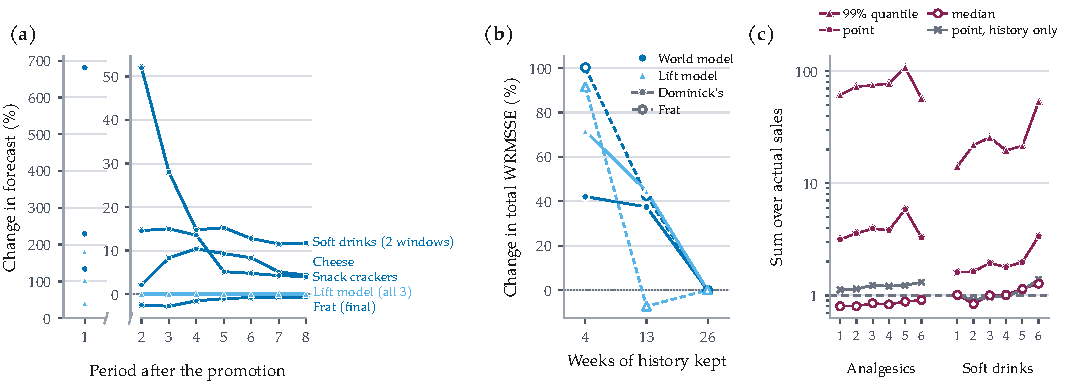
\includegraphics[width=\textwidth]{figs/fig_mechanism.pdf}
\caption{\textbf{The world model carries a promotion forward as further lift and
leans on the most recent weeks; Timestral given the plan puts extreme upper
quantiles on a few series.}
\textbf{(a)} Persistence: the change in the forecast, in percent, at each later
period after one promotion and a 20\% price cut are added in the first period
of the window, for the world model and the lift model (which has no carried
state, so its later change is zero by construction). \textbf{(b)} History
occlusion: the change in total WRMSSE, in percent, when only the last 4 or 13 of
the 26 weeks of history the models read are kept (26: nothing removed). \textbf{(c)} Timestral with the plan on two Dominick's
categories: the sum over all series of its median, its point forecast (the mean
of its quantiles) and its 99\% quantile, over actual sales, per rolling window;
log scale, dashed line at 1. Study B and the mechanism tests use the saved models
with no refitting; (c) from study F.}
\label{fig:mechanism}
\end{figure*}

All three trained models use the plan (Table~\ref{tab:perturbation}). With the
whole plan set to ``nothing planned'' the total error on Dominick's rises by
\rper{dom}{world}{wholeplan}{occlude}{total}\% for the world model,
\rper{dom}{lift}{wholeplan}{occlude}{total}\% for the lift model and
\rper{dom}{lgb}{wholeplan}{occlude}{total}\% for LightGBM, and the forecast in
planned periods changes by \rper{dom}{world}{wholeplan}{occlude}{units}\%,
\rper{dom}{lift}{wholeplan}{occlude}{units}\% and
\rper{dom}{lgb}{wholeplan}{occlude}{units}\%. Price carries more of it than
the promotion flag on Dominick's and Frat. On M5 prices rarely change, and the
plan inputs that matter are event and SNAP days: occluding SNAP days raises the
world model's total error by \rper{mfive}{world}{snap}{occlude}{total}\% and
LightGBM's by \rper{mfive}{lgb}{snap}{occlude}{total}\%, and occluding event days
by \rper{mfive}{world}{event}{occlude}{total}\% against
\rper{mfive}{lgb}{event}{occlude}{total}\%. The world model reads these
calendar inputs more than LightGBM does, which fits its lower error at the M5
total. On Frat the world model gets almost nothing from the
promotion flag once price is given (\rper{frat}{world}{promo}{occlude}{ixs}\%
item by store), while LightGBM and the lift model do.

Three tests on the saved world models show what the carried state does with
the plan. \emph{Timing}: shuffling the plan within each series, with its total
exposure unchanged, raises item-by-store error in cheese by
\rmech{che}{rolling}{world}{bottomchange}\% for the world model and
\rmech{che}{rolling}{lift}{bottomchange}\% for the lift model, and in snack
crackers by \rmech{sna}{rolling}{world}{bottomchange}\% and
\rmech{sna}{rolling}{lift}{bottomchange}\%: both use when the plan falls, and
the carried state adds little to that. \emph{Persistence}
(Figure~\ref{fig:mechanism}a): after a promotion and price cut added in the
first period, the world model's forecast stays higher in later periods, by
\rmech{sna}{rolling}{world}{persisth2}\% one period later in snack crackers and
\rmech{che}{rolling}{world}{persisth3}\% two periods later in cheese, falling
slowly. In categories where shoppers stock up, sales after a promotion dip; the
world model carries the promotion forward as further lift. On Frat the effect
is a small dip (\rmech{frat}{final}{world}{persisth2}\% one period later).
\emph{State}: a ridge read-out from the rolled state predicts sales in the
periods after the window no better than the same read-out from the state before
it ($R^2$ \rmech{che}{rolling}{world}{probeafterr2} against
\rmech{che}{rolling}{world}{probebeforer2} in cheese,
\rmech{mfive}{rolling}{world}{probeafterr2} against
\rmech{mfive}{rolling}{world}{probebeforer2} on M5).

On the weekly data the world model and the lift model read the last 26 weeks of
history, and the most recent weeks matter most (Figure~\ref{fig:mechanism}b):
keeping only the last 13 raises the Dominick's total error by
\rper{dom}{world}{historylast13}{occlude}{total}\% for the world model and
\rper{dom}{lift}{historylast13}{occlude}{total}\% for the lift model, and
keeping only the last 4 by \rper{dom}{world}{historylast4}{occlude}{total}\%
and \rper{dom}{lift}{historylast4}{occlude}{total}\%. On M5, keeping only the
last 28 days raises the world model's total error by
\rper{mfive}{world}{historylast28}{occlude}{total}\% and the lift model's by
\rper{mfive}{lift}{historylast28}{occlude}{total}\%.

\subsection{Pretrained models}
\label{sec:res-pretrained}

\begin{table*}[t]
\centering
\caption{\textbf{Timestral, released two days before this revision, is behind the ensemble on every data set, and
putting it in place of TimesFM helps only at the M5 total.} Mean WRMSSE over the rolling windows (Dominick's: mean
of the six categories). Timestral-28M, zero-shot, the mean of its 21 quantiles as the point forecast; with the plan as
known future inputs (TS+p) and from history alone (TS); TFM+p: TimesFM with the plan. Ens.: the ensemble; Ens.\,T:
Timestral with the plan in place of TimesFM with the plan; Ens.\,4: all four together. Study F, written down before it ran.}
\label{tab:timestral}
\footnotesize
\setlength{\tabcolsep}{3pt}
\begin{tabular}{l*{12}{r}}
\toprule
 & \multicolumn{6}{c}{\textbf{Item by store}} & \multicolumn{6}{c}{\textbf{Total}} \\
\cmidrule(lr){2-7}\cmidrule(lr){8-13}
\textbf{Data} & Ens. & Ens.\,T & Ens.\,4 & TFM+p & TS+p & TS & Ens. & Ens.\,T & Ens.\,4 & TFM+p & TS+p & TS \\
\midrule
Dominick's (six) & \textbf{0.612} & 0.916 & 0.821 & 0.613 & 1.565 & 0.728 & \textbf{0.672} & 3.729 & 2.858 & 0.807 & 10.788 & 2.121 \\
Frat & \textbf{0.549} & 0.623 & 0.595 & 0.578 & 0.864 & 0.792 & 0.337 & 0.501 & 0.407 & \textbf{0.327} & 1.048 & 0.484 \\
M5 & \textbf{0.834} & 0.846 & 0.842 & 0.842 & 0.894 & 0.861 & 0.706 & \textbf{0.609} & 0.699 & 1.035 & 1.025 & 1.014 \\
Favorita & \textbf{0.694} & 0.697 & \textbf{0.694} & 0.712 & 0.731 & 0.771 & 0.303 & \textbf{0.298} & 0.313 & 0.397 & 0.403 & 0.430 \\
\bottomrule
\end{tabular}
\end{table*}


TimesFM with the plan is the most accurate model not trained on the data, and
the plan matters to it: item by store it is ahead of TimesFM from history alone
on every data set where both ran except M5, where they tie
(Table~\ref{tab:rolling}), and most on the weekly
promotion-driven data (soft drinks \rv{sdr}{tfmplan}{ixs} against
\rv{sdr}{tfm}{ixs}). LightGBM is more accurate than it item by store on
\rcount{lgbbeatstfmplanixs} data sets and at the total on
\rcount{lgbbeatstfmplantotal}, and TimesFM with the plan is more accurate than
LightGBM on \rcount{tfmplanbeatslgbixs}.
Chronos-Bolt, from history alone, is behind TimesFM from history alone on every
data set item by store, and its total error in snack crackers is
\rv{sna}{chronos}{total}.

Timestral (study F, Table~\ref{tab:timestral}) is behind the ensemble on every
data set, at both levels. Given the plan it is behind TimesFM given the plan on
every data set except the M5 total, where they tie (\rsf{mfive}{tsplan}{total}
against \rsf{mfive}{tfmplan}{total}). Putting it in place of TimesFM makes the
ensemble less accurate on Dominick's and Frat, level at the Favorita total and
slightly less accurate item by store, and more
accurate only at the M5 total (\rsf{mfive}{enstimestral}{total} against
\rsf{mfive}{ens}{total}); as written down before it ran, the paper's ensemble is
unchanged and that swap is reported as a robustness result. The larger
Timestral-209M, run on Frat to check the model size, is less accurate than the
28M model (\rsf{frat}{tsbig}{ixs} against \rsf{frat}{tsplan}{ixs} item by
store).

On Dominick's Timestral with the plan forecasts several times total sales
(Figure~\ref{fig:mechanism}c). This is not a scale or input error: summed over
all series, its median is \rtail{ana}{tsplan}{median}{lo} to
\rtail{ana}{tsplan}{median}{hi} times actual sales in analgesics, and its
history-only point forecast \rtail{ana}{tsmean}{forecast}{lo} to
\rtail{ana}{tsmean}{forecast}{hi}. Given the plan, its 99\% quantile sums to
\rtail{ana}{tsplan}{q99}{lo} to \rtail{ana}{tsplan}{q99}{hi} times actual sales,
and because the point forecast is the mean of its quantiles, a few series carry
the error: the top 1\% of series by excess hold \rtail{ana}{tsplan}{share}{lo}\%
to \rtail{ana}{tsplan}{share}{hi}\% of it. The same happens more mildly in soft
drinks (99\% quantile \rtail{sdr}{tsplan}{q99}{lo} to
\rtail{sdr}{tsplan}{q99}{hi} times sales) and Frat
(\rtail{frat}{tsplan}{q99}{lo} to \rtail{frat}{tsplan}{q99}{hi}), and not on
the daily data. The forecast rule was not changed after the result. Timestral's
median would sit much closer to sales here, but it is fixed in advance to the
mean, as for Chronos-Bolt, because the median forecasts well below totals for
items that often sell nothing.

\subsection{A data set kept out of development}
\label{sec:res-favorita}

On Favorita, where nothing was tuned and every setting came from the M5
configuration, the ensemble has the lowest error at every level and is alone in
the model confidence set item by store (\rv{fav}{ens}{ixs} against
\rv{fav}{lgb}{ixs} for LightGBM and \rv{fav}{world}{ixs} for the world model);
at the total LightGBM (\rv{fav}{lgb}{total}) and the world model
(\rv{fav}{world}{total}) are in the set with it (\rv{fav}{ens}{total}). The world
model is behind LightGBM at every level, as on most of the other data sets, and
still adds to the ensemble item by store: without it the ensemble's error rises
by \rab{fav}{withoutworldmodel}{ixs}{meandiff}, and with the lift model in its
place by \rab{fav}{liftforworldmodel}{ixs}{meandiff}. The lift model is far
behind at the total (\rv{fav}{lift}{total}). Favorita has no prices, so its
weights are unit weights and its plan is promotions, holidays and paydays.

\subsection{Intervals and ranking}
\label{sec:res-intervals}

\begin{table*}[t]
\centering
\caption{\textbf{Rolling conformal intervals cover close to their level at item by store and somewhat less at the
total, and do not separate the models.} Scaled pinball loss (SPL, lower is better) and the share of actual sales
inside the 80\% and 95\% intervals, mean over the rolling windows after the first. Intervals from each model's own
scaled errors in the earlier windows of the data set, pooled over horizons where a level has fewer than 50 earlier
errors per horizon, ends rounded outwards to whole units except on Favorita (interval check of 16 October).}
\label{tab:intervals}
\footnotesize
\setlength{\tabcolsep}{2.6pt}
\begin{tabular}{l*{18}{r}}
\toprule
 & \multicolumn{9}{c}{\textbf{Item by store}} & \multicolumn{9}{c}{\textbf{Total}} \\
\cmidrule(lr){2-10}\cmidrule(lr){11-19}
 & \multicolumn{3}{c}{Ensemble} & \multicolumn{3}{c}{World} & \multicolumn{3}{c}{LightGBM}
 & \multicolumn{3}{c}{Ensemble} & \multicolumn{3}{c}{World} & \multicolumn{3}{c}{LightGBM} \\
\cmidrule(lr){2-4}\cmidrule(lr){5-7}\cmidrule(lr){8-10}\cmidrule(lr){11-13}\cmidrule(lr){14-16}\cmidrule(lr){17-19}
\textbf{Data} & SPL & 80 & 95 & SPL & 80 & 95 & SPL & 80 & 95 & SPL & 80 & 95 & SPL & 80 & 95 & SPL & 80 & 95 \\
\midrule
Cheese & 0.22 & 0.75 & 0.94 & 0.25 & 0.74 & 0.93 & 0.23 & 0.75 & 0.94 & 0.12 & 0.68 & 0.88 & 0.20 & 0.72 & 0.97 & 0.16 & 0.93 & 0.95 \\
Snack crackers & 0.23 & 0.74 & 0.94 & 0.24 & 0.73 & 0.94 & 0.23 & 0.73 & 0.93 & 0.53 & 0.60 & 0.72 & 0.80 & 0.57 & 0.60 & 0.42 & 0.75 & 0.88 \\
Soft drinks & 0.23 & 0.75 & 0.94 & 0.25 & 0.74 & 0.94 & 0.23 & 0.75 & 0.93 & 0.27 & 0.68 & 0.80 & 0.28 & 0.80 & 0.82 & 0.26 & 0.65 & 0.85 \\
Bottled juice & 0.23 & 0.73 & 0.93 & 0.26 & 0.72 & 0.93 & 0.24 & 0.73 & 0.93 & 0.15 & 0.82 & 0.93 & 0.20 & 0.80 & 0.95 & 0.15 & 0.93 & 0.97 \\
Analgesics & 0.25 & 0.91 & 0.98 & 0.25 & 0.91 & 0.98 & 0.24 & 0.91 & 0.98 & 0.25 & 0.85 & 0.88 & 0.29 & 0.85 & 0.95 & 0.27 & 0.88 & 0.95 \\
Frozen entrees & 0.18 & 0.69 & 0.93 & 0.18 & 0.69 & 0.93 & 0.17 & 0.70 & 0.93 & 0.12 & 0.90 & 0.97 & 0.12 & 0.88 & 1.00 & 0.10 & 0.82 & 0.90 \\
Frat & 0.20 & 0.87 & 0.97 & 0.22 & 0.87 & 0.97 & 0.21 & 0.87 & 0.97 & 0.11 & 0.75 & 0.96 & 0.15 & 0.83 & 0.88 & 0.14 & 0.62 & 0.83 \\
M5 & 0.32 & 0.94 & 0.98 & 0.33 & 0.94 & 0.98 & 0.33 & 0.94 & 0.98 & 0.18 & 0.71 & 0.94 & 0.19 & 0.76 & 0.86 & 0.14 & 0.80 & 0.98 \\
Favorita & 0.24 & 0.79 & 0.95 & 0.25 & 0.79 & 0.95 & 0.24 & 0.79 & 0.95 & 0.07 & 0.83 & 0.98 & 0.10 & 0.70 & 0.93 & 0.07 & 0.86 & 1.00 \\
\bottomrule
\end{tabular}
\end{table*}


The first conformal intervals covered far less than planned at the totals
(95\% intervals holding \rintold{mfive}{ens}{total}{coverage95} of actual sales
at the M5 total for the ensemble and \rintold{frat}{world}{total}{coverage95}
for the world model on Frat), because a level with one node has one earlier
error per horizon per window, so the 2.5\% and 97.5\% quantiles were the
smallest and largest of one to four numbers. With horizons pooled where errors
are few (Table~\ref{tab:intervals}, Figure~\ref{fig:decisions}b) the ensemble's 95\% interval holds
\rint{mfive}{ens}{total}{coverage95} at the M5 total and
\rint{frat}{ens}{total}{coverage95} on Frat. Item by store the 95\% intervals hold
0.93 to 0.98 of sales for all three models, and above 0.95 on M5 and Frat because
rounding a narrow interval outwards to a whole unit widens it; the pinball loss,
unchanged by rounding, is the measure to compare there, and it separates the
three models by at most 0.03 on every data set. Scored on their own
quantiles item by store, TFT's are level with the conformal intervals
(\rint{frat}{tft}{native}{spl} on Frat against \rint{frat}{ens}{ixs}{spl} for
the ensemble) and Chronos-Bolt's are behind them
(\rint{mfive}{chronos}{native}{spl} on M5 against \rint{mfive}{ens}{ixs}{spl}).

The ensemble also ranks item-by-store changes better than any single model
(Figure~\ref{fig:decisions}c). Across item-store series, the Spearman
correlation between forecast and actual change is \rrank{dom}{ens}{ixs}{spearman}
on Dominick's, \rrank{fav}{ens}{ixs}{spearman} on Favorita,
\rrank{frat}{ens}{ixs}{spearman} on Frat and \rrank{mfive}{ens}{ixs}{spearman}
on M5, above every single model in the check on each; of the tenth of
series it forecasts to grow most, \rrank{dom}{ens}{ixs}{topdecilehit},
\rrank{fav}{ens}{ixs}{topdecilehit}, \rrank{frat}{ens}{ixs}{topdecilehit} and
\rrank{mfive}{ens}{ixs}{topdecilehit} are in the actual top tenth, against
0.10 by chance. Over promoted periods LightGBM and the ensemble rank promotions best
(\rrank{dom}{lgb}{ixs}{promospearman} and \rrank{dom}{ens}{ixs}{promospearman}
on Dominick's). The ensemble's total forecast is within 6\% of actual sales on
every data source (\rrank{mfive}{ens}{ixs}{totalratio} on M5 is the furthest).

\subsection{Decisions and reconciliation}
\label{sec:res-decisions}
\label{sec:res-recon}

\begin{table*}[t]
\centering
\caption{\textbf{For category plans the world model alone has the lowest cost on \rcount{decworldcat} of eight data sets;
for store orders the ensemble or LightGBM has the lowest cost on every one.} Cost relative to seasonal naive (below 1 is better), mean over the rolling
windows. Category plan: absolute error of each category-by-store total over the window, weighted by dollar sales.
Store orders: order the model's 80\% interval quantile for each item, store and period; each unit over costs 1 and each
unit short costs 4. Simulations under stated costs, not business results. Bold: the lowest in the group.}
\label{tab:decisions}
\footnotesize
\setlength{\tabcolsep}{3.6pt}
\begin{tabular}{l*{10}{r}}
\toprule
 & \multicolumn{5}{c}{\textbf{Category plan}} & \multicolumn{5}{c}{\textbf{Store orders (ratio 0.8)}} \\
\cmidrule(lr){2-6}\cmidrule(lr){7-11}
\textbf{Data} & Ens. & World & Lift & LGB & TFM+p & Ens. & World & Lift & LGB & TFM+p \\
\midrule
Cheese & 0.26 & \textbf{0.12} & 0.16 & 0.30 & 0.36 & 0.52 & 0.55 & 0.57 & \textbf{0.52} & 0.62 \\
Snack crackers & 0.46 & \textbf{0.43} & 0.50 & 0.46 & 0.48 & 0.72 & 0.77 & 0.77 & \textbf{0.71} & 0.76 \\
Soft drinks & 0.19 & \textbf{0.08} & 0.14 & 0.17 & 0.33 & 0.59 & 0.61 & 0.64 & \textbf{0.57} & 0.69 \\
Bottled juice & 0.23 & \textbf{0.12} & 0.18 & 0.28 & 0.29 & \textbf{0.48} & 0.49 & 0.51 & 0.49 & 0.54 \\
Analgesics & 0.41 & 0.43 & 0.39 & \textbf{0.38} & 0.42 & 0.68 & 0.70 & 0.71 & \textbf{0.68} & 0.71 \\
Frozen entrees & 0.17 & \textbf{0.07} & 0.19 & 0.17 & 0.27 & 0.51 & 0.52 & 0.60 & \textbf{0.51} & 0.63 \\
Frat & \textbf{0.50} & 0.57 & 0.56 & 0.51 & 0.52 & \textbf{0.50} & 0.53 & 0.52 & 0.52 & 0.56 \\
M5 & 0.64 & \textbf{0.63} & 1.32 & 0.65 & 0.84 & \textbf{0.82} & 0.83 & 0.88 & 0.85 & 0.83 \\
\bottomrule
\end{tabular}
\end{table*}


\begin{figure*}[t]
\centering
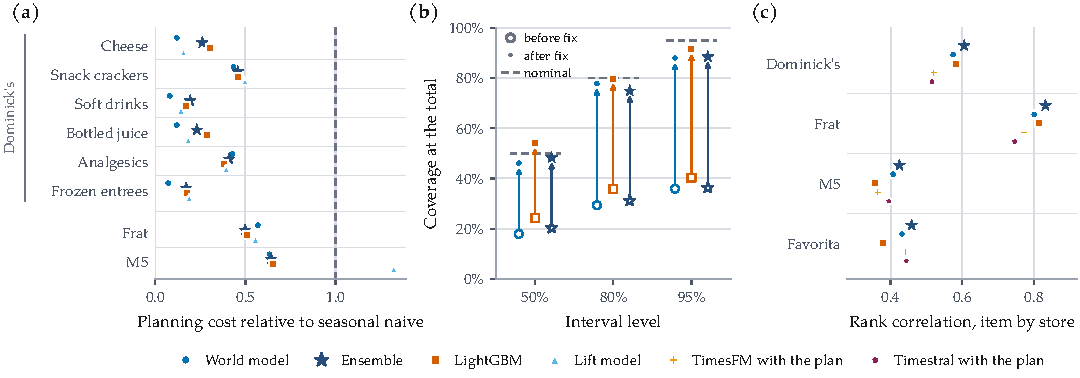
\includegraphics[width=\textwidth]{figs/fig_decisions.pdf}
\caption{\textbf{The world model has the lowest category-plan cost on most data
sets, pooling fixed the interval coverage at the totals, and the ensemble ranks
changes best.} \textbf{(a)} Category-plan cost relative to seasonal naive
(dashed line at 1), mean over the rolling windows. \textbf{(b)} Share of actual
sales inside the 50\%, 80\% and 95\% intervals at the chain total, mean over
the eight data sets scored both before the interval fix (open) and after it
(filled); dashes: the nominal level. \textbf{(c)} Spearman correlation across
item-store series between forecast and actual change, mean over the rolling
windows (Dominick's: over its six categories).}
\label{fig:decisions}
\end{figure*}

The two decisions point to different models (Table~\ref{tab:decisions},
Figure~\ref{fig:decisions}a). For the
category plan, the world model alone has the lowest cost on
\rcount{decworldcat} of eight data sets (\rcount{decworldcatlist}), at
\rdec{fre}{categoryplanning}{world} of seasonal naive's cost in frozen entrees
against \rdec{fre}{categoryplanning}{ens} for the ensemble and
\rdec{fre}{categoryplanning}{lgb} for LightGBM. Its category-by-store totals
over the window are close even where its item forecasts are behind LightGBM's.
For store orders
at a critical ratio of 0.8, LightGBM has the lowest cost on
\rcount{declgborder} (\rcount{declgborderlist}) and the ensemble on
\rcount{decensorder} (\rcount{decensorderlist}); the world model on none.

\begin{table}[t]
\centering
\caption{\textbf{Reconciled ETS forecasts are far behind the trained models; reconciling a trained model's item
forecasts with ETS above them helps on Frat and hurts on M5.} Mean WRMSSE over the rolling windows. MinT with a shrunk
covariance was computed only where the hierarchy has at most 6,000 nodes; on Frat it gave a total WRMSSE of
\rrec{frat}{etsmintshrink}{total}, a numerical failure not investigated further.}
\label{tab:reconcile}
\footnotesize
\setlength{\tabcolsep}{3pt}
\begin{tabular}{p{0.42\columnwidth}rrrr}
\toprule
 & \multicolumn{2}{c}{\textbf{Frat}} & \multicolumn{2}{c}{\textbf{M5}} \\
\cmidrule(lr){2-3}\cmidrule(lr){4-5}
\textbf{Method} & I$\times$S & Total & I$\times$S & Total \\
\midrule
ETS, bottom-up & 0.909 & 0.566 & 0.898 & 1.271 \\
ETS, top-down & 0.806 & 0.487 & 0.917 & 0.902 \\
ETS, OLS & 0.953 & 0.520 & 0.888 & 0.902 \\
ETS, WLS structural & 0.912 & 0.538 & 0.885 & 0.908 \\
ETS, WLS variance & 0.903 & 0.511 & 0.884 & 0.946 \\
ETS, MinT shrink & 0.926 & 247.170 & -- & -- \\
LightGBM + ETS, WLS variance & 0.581 & 0.304 & 0.855 & 0.763 \\
World model + ETS, WLS variance & 0.602 & 0.343 & 0.849 & 0.754 \\
\midrule
LightGBM, unreconciled & 0.570 & 0.360 & 0.861 & 0.693 \\
World model, unreconciled & 0.595 & 0.457 & 0.851 & 0.609 \\
Ensemble, unreconciled & 0.549 & 0.337 & 0.834 & 0.706 \\
\bottomrule
\end{tabular}
\end{table}


Reconciliation does not replace a model trained on the plan
(Table~\ref{tab:reconcile}). The best reconciled ETS forecast on Frat is
top-down, at \rrec{frat}{etstopdown}{ixs} item by store against
\rv{frat}{lgb}{ixs} for LightGBM. Combining a trained model's item forecasts
with ETS above them by weighted least squares lowers the Frat total error
(LightGBM \rrec{frat}{lightgbmwithetswlsvar}{total} against
\rv{frat}{lgb}{total} unreconciled; world model
\rrec{frat}{worldmodelwithetswlsvar}{total} against \rv{frat}{world}{total})
and raises the M5 total error (world model
\rrec{mfive}{worldmodelwithetswlsvar}{total} against
\rv{mfive}{world}{total}). MinT with a shrunk covariance gave a total WRMSSE of
\rrec{frat}{etsmintshrink}{total} on Frat, a numerical failure we did not
investigate further.

\subsection{The final windows of the first version}
\label{sec:res-final}

\begin{table*}[t]
\centering
\caption{\textbf{On M5 the best model depends on the level scored and on the month.} WRMSSE on the four 28-day
windows (lower is better), mean over seeds; seeds per window in the second column. All: the 12 levels together;
Total: the chain total; I$\times$S: item by store. The lowest value in each column is in bold. TimesFM with the
plan has no recorded total. The lift model's April mean includes one failed seed (2.603 overall;
\S\ref{sec:failures}).}
\label{tab:m5}
\footnotesize
\setlength{\tabcolsep}{3.6pt}
\begin{tabular}{lc*{12}{r}}
\toprule
 & & \multicolumn{3}{c}{\textbf{29 Feb to 27 Mar}} & \multicolumn{3}{c}{\textbf{28 Mar to 24 Apr}} & \multicolumn{3}{c}{\textbf{25 Apr to 22 May (practice)}} & \multicolumn{3}{c}{\textbf{23 May to 19 Jun (test)}} \\
\cmidrule(lr){3-5}\cmidrule(lr){6-8}\cmidrule(lr){9-11}\cmidrule(lr){12-14}
\textbf{Model} & \textbf{Seeds} & All & Total & I$\times$S & All & Total & I$\times$S & All & Total & I$\times$S & All & Total & I$\times$S \\
\midrule
World model & 3/3/3/3 & \textbf{0.642} & \textbf{0.398} & 0.851 & \textbf{0.555} & \textbf{0.283} & 0.833 & 0.656 & 0.535 & 0.834 & 0.638 & 0.379 & 0.897 \\
Lift model & 3/3/3/3 & 0.664 & 0.427 & 0.846 & 1.246 & 0.964 & 0.834 & 0.713 & 0.623 & 0.832 & 0.663 & 0.368 & 0.896 \\
LightGBM & 3/3/1/3 & 0.709 & 0.578 & 0.873 & 0.557 & 0.351 & 0.846 & 0.715 & 0.659 & 0.847 & \textbf{0.547} & \textbf{0.247} & 0.905 \\
Graph model & 3/3/3/3 & 0.778 & 0.621 & 0.878 & 0.644 & 0.493 & 0.845 & \textbf{0.641} & \textbf{0.455} & 0.851 & 0.673 & 0.412 & 0.909 \\
TimesFM & 1/1/1/1 & 0.854 & 0.830 & \textbf{0.836} & 0.819 & 0.786 & \textbf{0.828} & 0.896 & 0.930 & \textbf{0.828} & 0.729 & 0.558 & 0.885 \\
TimesFM with the plan & 1/1/1/1 & 0.858 & -- & 0.837 & 0.772 & -- & 0.829 & 0.929 & -- & 0.830 & 0.719 & -- & \textbf{0.883} \\
Seasonal naive & 1/1/1/1 & 0.889 & 0.658 & 1.121 & 0.923 & 0.668 & 1.126 & 0.870 & 0.751 & 1.100 & 0.847 & 0.560 & 1.176 \\
\bottomrule
\end{tabular}
\end{table*}

\begin{table*}[t]
\centering
\caption{\textbf{On the promotion-driven weekly data, models that see the plan lead, and which one leads
changes by category.} WRMSSE on the final 8 weeks (lower is better). World model, lift model and LightGBM:
mean of three seeds, settings fixed on the development windows. TimesFM and TimesFM with the plan: one run each,
added after the final tests. The lift model was run on Frat only. The lowest value in each row and group is in bold.}
\label{tab:finals}
\footnotesize
\setlength{\tabcolsep}{4pt}
\begin{tabular}{l*{10}{r}}
\toprule
 & \multicolumn{5}{c}{\textbf{All levels}} & \multicolumn{5}{c}{\textbf{Item by store}} \\
\cmidrule(lr){2-6}\cmidrule(lr){7-11}
\textbf{Data} & World & Lift & LightGBM & TimesFM & TimesFM+plan & World & Lift & LightGBM & TimesFM & TimesFM+plan \\
\midrule
Frat & 0.681 & 0.714 & \textbf{0.549} & 0.965 & 0.686 & 0.665 & 0.677 & \textbf{0.608} & 0.827 & 0.641 \\
\addlinespace[2pt]
\multicolumn{11}{l}{\itshape Dominick's} \\
Cheese & 0.897 & -- & 0.708 & 0.829 & \textbf{0.545} & 0.715 & -- & 0.702 & 0.792 & \textbf{0.699} \\
Snack crackers & 0.448 & -- & \textbf{0.412} & 0.468 & 0.475 & 0.608 & -- & \textbf{0.596} & 0.640 & 0.614 \\
Soft drinks & \textbf{0.830} & -- & 0.989 & 1.070 & 0.974 & 0.734 & -- & \textbf{0.652} & 0.895 & 0.780 \\
Bottled juice & 0.987 & -- & 0.994 & \textbf{0.940} & 0.990 & 0.816 & -- & \textbf{0.750} & 0.782 & 0.754 \\
Analgesics & \textbf{0.867} & -- & 0.978 & 1.009 & 0.889 & \textbf{0.713} & -- & 0.714 & 0.790 & 0.742 \\
Frozen entrees & 0.485 & -- & \textbf{0.478} & 0.563 & 0.566 & 0.557 & -- & \textbf{0.529} & 0.682 & 0.599 \\
\bottomrule
\end{tabular}
\end{table*}

\begin{table*}[t]
\centering
\caption{\textbf{On the single final windows the ensemble is lowest or within \rcount{finalsgap} of the lowest item by
store on every data set, and the order at the total changes from data set to data set.} WRMSSE on the final
window of each data set (lower is better; on M5 the official test month). One fit (seed~1) per trained model, so the world
model and LightGBM differ slightly from the three-seed means of Tables~\ref{tab:m5} and~\ref{tab:finals}. Bold:
lowest in the group.}
\label{tab:finalsnew}
\footnotesize
\setlength{\tabcolsep}{3pt}
\begin{tabular}{l*{14}{r}}
\toprule
 & \multicolumn{7}{c}{\textbf{Item by store}} & \multicolumn{7}{c}{\textbf{Total}} \\
\cmidrule(lr){2-8}\cmidrule(lr){9-15}
\textbf{Data} & Ens. & World & Lift & LGB & TFM+p & Chr. & TFT & Ens. & World & Lift & LGB & TFM+p & Chr. & TFT \\
\midrule
Cheese & \textbf{0.675} & 0.712 & 0.756 & 0.699 & 0.704 & 0.807 & 0.731 & 0.753 & 1.064 & 0.997 & 0.768 & 0.531 & 1.009 & \textbf{0.522} \\
Snack crackers & \textbf{0.585} & 0.610 & 0.620 & 0.603 & 0.624 & 0.661 & 0.621 & 0.334 & 0.484 & 0.302 & 0.317 & 0.362 & 0.327 & \textbf{0.219} \\
Soft drinks & 0.674 & 0.709 & 0.772 & \textbf{0.655} & 0.780 & 0.912 & 0.849 & 1.065 & \textbf{0.891} & 0.920 & 1.238 & 1.140 & 1.385 & 1.228 \\
Bottled juice & 0.760 & 0.849 & 0.807 & 0.756 & \textbf{0.754} & 0.785 & 0.775 & 1.111 & 1.019 & 1.190 & 1.171 & 1.172 & 1.046 & \textbf{1.015} \\
Analgesics & \textbf{0.710} & 0.712 & 0.714 & 0.716 & 0.742 & 0.802 & 0.770 & 1.236 & 1.186 & 1.280 & 1.407 & 1.149 & 1.454 & \textbf{0.878} \\
Frozen entrees & 0.543 & 0.574 & 0.563 & \textbf{0.530} & 0.599 & 0.692 & 0.557 & 0.454 & 0.423 & \textbf{0.404} & 0.438 & 0.537 & 0.536 & 0.414 \\
Frat & \textbf{0.604} & 0.671 & 0.662 & 0.613 & 0.644 & 0.856 & 0.702 & 0.586 & 0.681 & 0.698 & \textbf{0.523} & 0.677 & 1.222 & 0.818 \\
M5 & \textbf{0.881} & 0.896 & 0.896 & 0.905 & 0.883 & 0.899 & -- & \textbf{0.240} & 0.363 & 0.424 & 0.245 & 0.556 & 1.007 & -- \\
\bottomrule
\end{tabular}
\end{table*}


The first version scored each data set once, on its final window, and its
findings stand: on M5 the most accurate model depended on the level and the
month (Table~\ref{tab:m5}), and on Dominick's and Frat on the category
(Table~\ref{tab:finals}). On M5, TimesFM given only history was the most
accurate single model item by store in all four months (\mTfmTestIxs{} on the
test month, against \mWorldTestIxs{} for the world model and \mLgbTestIxs{} for
LightGBM), while the plan-aware models were far more accurate at the totals. The
official test month was the only one of four in which LightGBM was the most
accurate over all levels (\mLgbTestOverall{} against \mWorldTestOverall), so a
comparison on that month alone would have ranked it first. Run on the final
windows (Table~\ref{tab:finalsnew}), the ensemble is lowest or within
\rcount{finalsgap} of the lowest item by store on every data set, which agrees
with the rolling windows.

\begin{figure*}[t]
\centering
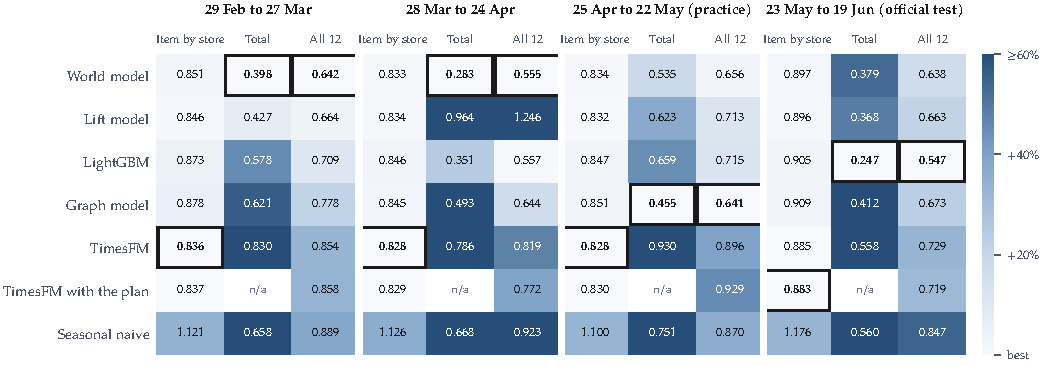
\includegraphics[width=\textwidth]{figs/fig_m5_heat.pdf}
\caption{\textbf{On the M5 final windows, TimesFM from history alone had the
lowest item-by-store error of the single models in every month; at the total and
over all levels the plan-aware models did, and which one changed by month.}
WRMSSE of every single model, four windows, three levels; cell shade: how far
above the lowest value in its column (white: the lowest, outlined). Trained
models: mean of three seeds. The lift model's April mean includes one failed
seed (\S\ref{sec:dropped}).}
\label{fig:m5heat}
\end{figure*}

\paragraph{How much the plan matters}
On M5, where prices rarely change, giving TimesFM the plan changed its
item-by-store error by at most 0.002 in any month. On Dominick's, where promoted
weeks carry \promoShareLo\% to \promoShareHi\% of a category's units, TimesFM
without the plan forecast \promoTfmLo\% to \promoTfmHi\% of promoted-week sales
and with it \promoTfmPlanLo\% to \promoTfmPlanHi\%
(Figure~\ref{fig:planarrows}a). The trained plan-aware models also fell short in
promoted weeks: the world model forecast \promoWorldLo\% to \promoWorldHi\% of
promoted-week sales and LightGBM \promoLgbLo\% to \promoLgbHi\%.

\begin{figure*}[t]
\centering
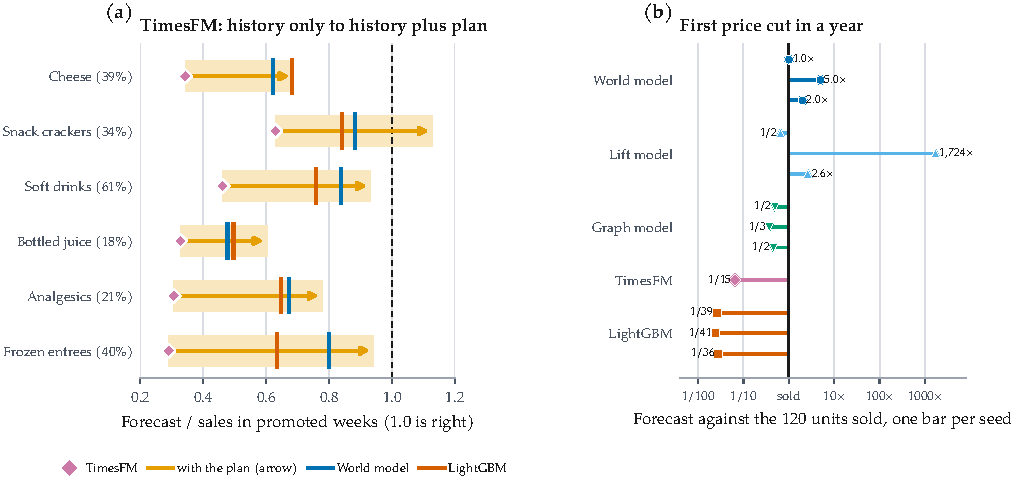
\includegraphics[width=\textwidth]{figs/fig_plan_arrows.pdf}
\caption{\textbf{Given the plan, TimesFM closes most of its promoted-week
shortfall; for a price cut history has not shown, plan-aware models respond and
history-only models do not.} \textbf{(a)} Forecast against sales in the promoted
weeks of the final 8 weeks, by Dominick's category (promoted weeks' share of the
category's units in brackets): TimesFM from history alone (diamond) to TimesFM
with the plan (arrow head), with the world model and LightGBM (ticks). \textbf{(b)}
HOUSEHOLD\_1\_146 in the four M5 stores where it had its first price cut in a year
(5.98 to 4.50 for one week) inside the April window: each seed's forecast over
the 28 days against the \cutSold{} units sold, log scale.}
\label{fig:planarrows}
\end{figure*}

\paragraph{First-time price cuts}
In the April M5 window, HOUSEHOLD\_1\_146 had sold almost nothing for a year at
5.98, then sold \cutSold{} units in four stores over a window that held a
one-week cut to 4.50 (Figure~\ref{fig:planarrows}b). Models working from history
forecast almost nothing: LightGBM \cutLgb{} units across seeds, TimesFM
\cutTfm. The world model, which reads the cut through its plan, forecast
\cutWorld; the graph model \cutGraph; the lift model \cutLift. How large the
response should be is not fixed by the data: the world-model seeds differ by a
factor of five, and one lift-model seed forecast over 200,000 units.

% =====================================================================
\section{What was tried and dropped}
\label{sec:dropped}

We report the failures at the same length as the results.
Table~\ref{tab:dropped} lists what this revision tried and did not keep, and
Table~\ref{tab:ledger} what the first version did.

\begin{table*}[t]
\centering
\caption{\textbf{What the revision tried and did not keep.} Each was written
down with its pass rule before it ran. dev.: the development windows of the six
Dominick's categories. After promotion: forecast over actual in the two periods
after a promotion.}
\label{tab:dropped}
\footnotesize
\renewcommand{\arraystretch}{1.15}
\begin{tabular}{p{0.26\textwidth}p{0.21\textwidth}p{0.45\textwidth}}
\toprule
\textbf{Change or model} & \textbf{Where tested} & \textbf{Result} \\
\midrule
Stock term on the world model (study C) & Dominick's dev., seed 1 & Overall worse than the world model in three of six categories \\
Plan of the two periods before, on the lift model (study C) & Dominick's dev., seed 1 & Overall worse than the world model in three of six \\
Stock term on the lift model (study C) & Dominick's dev., then rolling & Passed on development (after promotion \rpan{dev}{sdr}{liftstock}{mean}{afterpromofa} soft drinks, \rpan{dev}{sna}{liftstock}{mean}{afterpromofa} snack crackers); on the rolling windows \rpan{rol}{sdr}{liftstock}{roll}{afterpromofa} and \rpan{rol}{sna}{liftstock}{roll}{afterpromofa}, against \rpan{rol}{sdr}{worldmodel}{roll}{afterpromofa} and \rpan{rol}{sna}{worldmodel}{roll}{afterpromofa} for the world model \\
Weight 3 on periods after a promotion (study E) & Dominick's dev., seed 1 & Error after promotion lower in all six (soft drinks \raft{sdr}{worldmodel}{afterpromoerr} to \raft{sdr}{afterpromow2}{afterpromoerr}); overall worse in four (snack crackers \raft{sna}{worldmodel}{overall} to \raft{sna}{afterpromow2}{overall}) \\
Weight 6 on periods after a promotion (study E) & Dominick's dev., seed 1 & Overall worse in four; snack crackers after promotion \raft{sna}{afterpromow5}{afterpromofa} \\
Fitted ensemble weights (study A) & All nine, rolling & Better than equal weights in \rcount{fittedwins} of \rcount{fittedn} comparisons, worse in \rcount{fittedlosses} \\
Timestral in place of TimesFM (study F) & All four sources, rolling & Worse on Dominick's and Frat; better at the M5 total only \\
Timestral-209M (study F) & Frat, rolling & Less accurate than 28M; too slow for the other data sets \\
MinT, shrunk covariance & Frat, rolling & Total WRMSSE \rrec{frat}{etsmintshrink}{total}; not investigated \\
\bottomrule
\end{tabular}
\end{table*}

\begin{table*}[t]
\centering
\caption{\textbf{Every change and comparison model that did not become a default.} Overall WRMSSE unless
stated; ``against'' gives the default it was compared with on the same window. dev.: development windows before
the final 8 weeks. Practice: the M5 window 25 April to 22 May 2016. Each row is a section of
\texttt{results/README.md} with its run folders.}
\label{tab:ledger}
\footnotesize
\begin{tabular}{p{0.30\textwidth}p{0.28\textwidth}p{0.34\textwidth}}
\toprule
\textbf{Change or model} & \textbf{Where tested} & \textbf{Result} \\
\midrule
Twice the training steps & Dominick's (6) and Frat, dev., 3 seeds & Better in 2, worse in 3, level or mixed in 2 \\
Weekday as seven inputs & M5 practice, seed 1 & 0.653 against 0.646 \\
Event kinds (with weekday) & M5 practice, seed 1 & 0.646 against 0.646 \\
60,000 training steps & M5 practice, seed 1 & 0.642 against 0.646; gain below seed range 0.029 \\
Item level against past-year level & M5 practice, seed 1 & 0.680 against 0.646 \\
Totals term in the loss & Dominick's analgesics, dev. & 0.819 against 0.683; total 8\% under \\
Negative binomial likelihood & Frat, analgesics, dev. & Level \\
Plan split, latent check, near-week weighting & Frat, dev., 5 seeds & 0.417 to 0.427 against 0.408 \\
Own forecast fed into the roll-forward & Dominick's (6), dev. & Worse overall in 4 of 6 \\
Item role labels & Dominick's (6), dev. & No effect on LightGBM; snack crackers 2.422 for the world model \\
Averaging three fits & M5 practice, seed 1 & 0.665 against 0.656 (kept on Dominick's) \\
Graph model over product attributes & M5, four windows, 3 seeds & Level with LightGBM item by store \\
TimesFM, median output & M5, four windows & Overall 1.71 to 1.88; totals 27\% to 31\% under \\
Lift model (no roll-forward) & M5, four windows, 3 seeds & One seed failed in April (2.603) \\
\bottomrule
\end{tabular}
\end{table*}


\paragraph{The forecast after a promotion}
The persistence test showed the world model carrying a promotion forward as
further lift where shoppers stock up. Studies C and E tried to give the dip a
route. A stock term, one number per item that builds with sales above the
item's level, decays by a learnt share and lowers later sales by a learnt amount
that cannot be negative, made the world model worse overall in three of six
categories on the development windows. On the lift model it passed the
development rule, but on the rolling windows it did not fix the after-promotion
forecast (soft drinks \rpan{rol}{sdr}{liftstock}{roll}{afterpromofa} with it,
\rpan{rol}{sdr}{lift}{roll}{afterpromofa} for the plain lift model,
\rpan{rol}{sdr}{worldmodel}{roll}{afterpromofa} for the world model). A loss
weight on the periods after a promotion lowered the error there in all six
categories and made the overall score worse in four. None became a default. The
reason given for study C also needed a correction: the 1.32 and 1.33
after-promotion ratios that prompted it came from an earlier world-model
version; the final world model was at 1.00 and 1.04 on those windows.

\paragraph{A seed that never reached single fits, and noise as large as the
effects}
Stage 2 of study C repeated each configuration with seeds 2 and 3 and got
identical scores in all twelve runs. Single-fit configurations whose settings
named no seed trained with seed 0 for every run seed; the seed now reaches the
model, and the results already recorded are those of seed 0 (each manifest
records its commit). The repeat also showed that two runs of the same
configuration on different Colab machines differ by as much as the variants
being tested: the world model's overall score in snack crackers was
\rpan{dev}{sna}{worldmodel}{a}{overall} on one machine and
\rpan{dev}{sna}{worldmodel}{b}{overall} on another. Study E therefore reran the
world model in the same job as the variants it was compared with. The rolling
windows, being one fit per model, carry this noise; the paired tests over
windows absorb part of it, not all.

\paragraph{A lift-model seed that broke on five series}
In the April M5 final window, lift-model seed 2 scored \mLiftAprSeedBOverall{}
over all levels against \mLiftAprSeedAOverall{} and \mLiftAprSeedCOverall{} for
seeds 1 and 3, and forecast \liftSeedTwoForecast{} units against
\liftSeedTwoSold{} sold. Five item-store series hold all of the excess, each with
its first price cut in a year inside the window; the seed read the cuts as lifts
up to the model's bound. Item by store, weighted by dollar sales, the failure is
invisible (\mLiftAprIxs); at the totals it dominates. The world model did not
fail on these series in any seed.

\begin{figure*}[t]
\centering
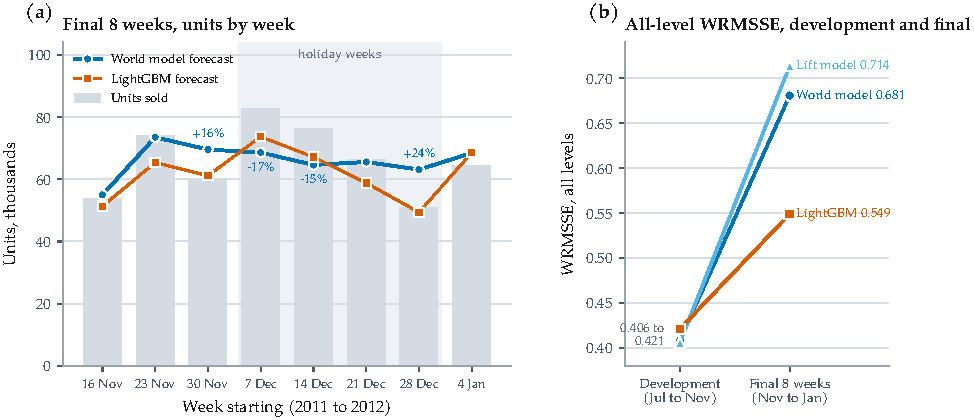
\includegraphics[width=\textwidth]{figs/fig_frat_story.pdf}
\caption{\textbf{On the Frat final window the world model got the 8-week total
right and missed the holiday shape, which the development windows did not
contain.} \textbf{(a)} Units sold each week of the final window over all
item-stores (bars), and the weekly forecasts of the world model and LightGBM,
three seeds averaged; labels: the world model's largest weekly misses.
\textbf{(b)} All-level WRMSSE on the development windows and on the final 8 weeks.}
\label{fig:fratstory}
\end{figure*}

\paragraph{Frat holiday weeks}
On the Frat development windows the world model, lift model and LightGBM were
level (0.406 to 0.421). On the final 8 weeks the world model fell to
\fWorldFratOverall{} against \fLgbFratOverall{} for LightGBM. The final weeks
are the holiday period, which the development windows did not contain
(Figure~\ref{fig:fratstory}); the world model's 8-week total is right (forecast
against sales \fWorldFratFa) but it is 15\% to 17\% under in the two December
peak weeks. LightGBM, with week-of-year and month inputs and the previous
holiday season in its training data, follows that shape more closely.

\paragraph{TimesFM's default output}
TimesFM's default point forecast is the median. For an item that sells nothing
on most days the median is near zero while the mean is not, so the median
forecast is 27\% to 31\% below M5 totals in every month. The mean output, used
throughout, does not have the problem.

% =====================================================================
\section{Discussion}
\label{sec:discussion}

A retailer that knows its plan should forecast items with an equal-weight
average of a plan-aware world model, a tree model and a pretrained model given
the plan, and should check the category totals against the world model alone
(Table~\ref{tab:advice}).

\begin{table*}[t]
\centering
\caption{\textbf{Each decision has its own level, and the results point to a
forecast for each.}}
\label{tab:advice}
\footnotesize
\renewcommand{\arraystretch}{1.2}
\begin{tabular}{p{0.23\textwidth}p{0.18\textwidth}p{0.51\textwidth}}
\toprule
\textbf{Decision} & \textbf{Level} & \textbf{What the results say} \\
\midrule
Store orders and inventory & Item by store, day or week & The ensemble or LightGBM: lowest order cost on every data set; the ensemble lowest item-by-store error on \rcount{enslowestixs} of nine \\
Promotion, price change, supplier funding & Item by week, under a planned change & A model that reads the plan; history alone forecasts \promoTfmLo\% to \promoTfmHi\% of promoted-week sales. Check forecasts after a promotion in categories where shoppers stock up: the world model carries the lift forward \\
Category sales, units and margin plans & Category or chain, week or month & The world model alone: lowest category-plan cost on \rcount{decworldcat} of eight; the ensemble at the total is in the confidence set everywhere \\
Choosing a model & Any & Score several windows with paired tests; one test month reversed the ranking on M5, and runs on different machines differed by as much as the changes tested \\
Adopting a new pretrained model & Any & Check its totals and its upper quantiles before use; Timestral's tails made its mean forecast several times sales on weekly data \\
\bottomrule
\end{tabular}
\end{table*}

\paragraph{Why an equal-weight ensemble}
The three members fail in different places. LightGBM is the most accurate single
model item by store on most data sets and the member the ensemble can least do
without. TimesFM with the plan brings a pretrained view of each series' history.
The world model has the lowest category-plan cost on \rcount{decworldcat} of
eight data sets, and the ensemble without it is less accurate item by store on
\rcount{withoutworldmodelixsens}. An average of three models whose errors
differ is more accurate item by store than any of them on
\rcount{enslowestixs} of nine data sets, and equal weights are as good as weights fitted on a few earlier
windows, as the forecast combination literature leads one to
expect~\cite{smithwallis2009,wang2023}.

\paragraph{What the carried state adds}
Against the lift model, which differs only in the carried state, the world model
is level on its own in most data sets, adds to the ensemble beyond the lift
model on \rcount{liftforworldmodelixsens} data sets item by store and
\rcount{liftforworldmodeltotalens} at the total, and has a lower category-plan
cost than the lift model on \rcount{worldbeatsliftcat} of eight. The carried state holds the plan (Figure~\ref{fig:readback}), but the
rolled state does not predict sales beyond the window better than the state
before it, and it carries a promotion forward as more lift rather than a dip.
On these data the case for the carried state is what it adds to an ensemble and
to category totals, not item accuracy on its own.

\paragraph{Two cautions}
A plan-driven forecast responds to plans unlike history with a size the data do
not fix: one lift-model seed and Timestral's upper quantiles both produced
forecasts many times any sale. And a forecast that is accurate item by store
can be several percent off the category total, which is the number a merchant
plans against.

% =====================================================================
\section{Limitations and threats to validity}
\label{sec:limitations}

\paragraph{Windows and seeds}
Trained models are one fit each in the rolling windows, and runs of one
configuration on different machines differed by as much as some differences
tested (\S\ref{sec:dropped}). Four to six windows per data set give wide
intervals across windows, so ``level'' often means ``not separated''. Single-fit
runs before 16 October trained with seed 0 whatever seed was named.

\paragraph{Studies added after the main results}
Studies A to F were added after the rolling results were read. Each was written
down before it ran, but which studies to run was chosen knowing that the
ensemble came first. Timestral was run at 28M parameters, not 209M, because the
larger model was too slow, a change made before any Timestral result.

\paragraph{Comparison models}
TFT was not run on M5 or Favorita, and Chronos-Bolt and TimesFM from history
alone not on Favorita. TimesFM with the plan fits its linear plan model within
groups of 2,048 series. Pretrained models are used as published with their point
forecast fixed in advance (the mean), which for Timestral was the wrong choice on
weekly data.

\paragraph{What lift means}
Merchants promote in weeks they expect to sell well, so part of a measured lift
is good timing. The lift is what the forecast attributes to the plan, not what
the plan caused. Our companion audit~\cite{paper2} measures the gap in generated
store data where the true lifts are known: the world model's and LightGBM's
lifts were a third too large while every check against the model passed. Plan
responses in this paper, including the perturbation tests, are forecasts, not
causal estimates.

\paragraph{What the data do not record}
None of the data sets records stock, so a sell-out looks like low demand; or
shelf space. Favorita records no prices. The data were collected between 1989
and 2017 and their plan inputs differ, so the results compare models within each
data set. The decision costs are simulations under stated costs.

% =====================================================================
\section{Conclusion}
\label{sec:conclusion}

An equal-weight ensemble of a world model, LightGBM and TimesFM given the plan
is the most accurate item-by-store forecast on rolling windows of four public
retail data sets, including one kept out of development, and it is never less
accurate than LightGBM or the world model by a paired test. The world model
adds to it on some data sets, and its carried state on fewer; on its own it is
behind LightGBM item by store and gets category totals right. Every trained model
uses the plan, the world model carries promotions forward as further lift, and a
pretrained model released this month needs its tails checked before use.
Retail forecasts should be chosen by the decision they feed, at that decision's
level, over several windows with paired tests, with the losing models stated.

\section{Reproducibility and compute}
\label{sec:repro}

\paragraph{Records}
All code, configuration files and tests are in the repository. A run refuses to
start on uncommitted code and writes a manifest holding the code commit, the
full configuration and its checksum, the seed, checksums of every data file
read, package versions, the machine and run times. The manifest and scores of
the \nPromotedRuns{} final-window runs are committed under
\nolinkurl{results/promoted/}. The revision's analyses of saved forecasts are
committed as tables under \nolinkurl{results/paper1_revision/tables/}, with the
per-window scores of study F under \nolinkurl{results/paper1_revision/scores/};
the plan and every amendment are in \nolinkurl{docs/PAPER1_REVISION_PLAN.md}.
\texttt{make} in \texttt{paper/} rebuilds every figure, table and quoted number
from these files (26 seconds from a clean copy of the repository on two CPU
cores, 17 October 2026), and a quoted revision number that is missing from them stops
the build. One table was transcribed from a console run rather than written by a
script: Timestral's quantile sums (\nolinkurl{studyF_tails.csv}), from
\nolinkurl{scripts/timestral_tails.py}. Forecast files and model checkpoints are
kept outside the repository with their checksums recorded.

\paragraph{Compute}
Every run used one Google Colab machine: an NVIDIA \computeGpu{} with
\computeGpuMem{}~GB of memory, a \computeCores-core \computeCpu{} and
\computeRam{}~GB of memory, PyTorch \computeTorch{} with CUDA \computeCuda.
Table~\ref{tab:compute} gives the run time of every timed final and comparison
run of the first version: \computeRuns{} runs and \computeHours{} machine-hours.
The revision's rolling windows, studies and analyses were not timed as a whole;
from the working sessions we estimate about 60 further machine-hours on T4 and
L4 GPUs, of which study F took about 12. This is an estimate, not a record.

\begin{table}[t]
\centering
\caption{\textbf{Run times of the final and comparison runs, from their manifests.} Wall-clock minutes per
run (data loading, training, forecasting and scoring) and hours in total, on one Google Colab machine with an NVIDIA Tesla T4 (LightGBM uses its CPU). Dominick's:
six categories together; a Dominick's world-model run averages three fits. Two M5 runs resumed after the
Colab runtime dropped record only the resumed part (the shortest values in their rows). Not counted: runs saved before
run times were recorded, the development study, and TimesFM on Dominick's and Frat.}
\label{tab:compute}
\footnotesize
\setlength{\tabcolsep}{3.5pt}
\begin{tabular}{llrrlr}
\toprule
\textbf{Data} & \textbf{Model} & \textbf{Runs} & \textbf{Median} & \textbf{Range} & \textbf{Hours} \\
\midrule
M5 & World model & 9 & 101.5 & 37.3 to 103.2 & 14.0 \\
M5 & Lift model & 9 & 88.7 & 10.3 to 94.6 & 12.2 \\
M5 & LightGBM & 9 & 78.1 & 76.5 to 79.9 & 11.7 \\
M5 & Graph model & 12 & 7.2 & 7.2 to 7.5 & 1.5 \\
M5 & TimesFM & 8 & 3.9 & 3.8 to 4.1 & 0.5 \\
M5 & Seasonal naive & 2 & 1.3 & 1.2 to 1.3 & 0.0 \\
Dominick's & World model & 18 & 9.2 & 9.0 to 10.6 & 2.8 \\
Dominick's & LightGBM & 18 & 4.6 & 3.1 to 11.5 & 1.7 \\
Frat & World model & 3 & 2.2 & 2.2 to 2.2 & 0.1 \\
Frat & Lift model & 3 & 2.0 & 1.9 to 2.0 & 0.1 \\
Frat & LightGBM & 3 & 1.5 & 1.5 to 1.6 & 0.1 \\
\midrule
\multicolumn{5}{l}{All 94 timed runs} & 44.7 \\
\bottomrule
\end{tabular}
\end{table}


\section{Data, code and licence}
\label{sec:licence}

\paragraph{Data}
M5 is available from the competition's Kaggle page~\cite{m5accuracy};
Dominick's from the Kilts Center for Marketing, University of Chicago Booth
School of Business~\cite{dominicks}; Breakfast at the Frat from
dunnhumby~\cite{frat}; Corporaci\'on Favorita from its Kaggle
competition~\cite{favorita}. Each is obtained from its provider under the
provider's own terms. No data is redistributed with the code.

\paragraph{Code}
The code is at
\url{https://github.com/Kar488/retail-world-models}.

\paragraph{Licence}
The code is licensed under the PolyForm Noncommercial License~1.0.0. The
manuscript text, figures and tables are licensed under Creative Commons
Attribution-NonCommercial~4.0 International (CC~BY-NC~4.0). Commercial use of
either needs a separate licence from the author.

\begin{thebibliography}{99}
\footnotesize
\setlength{\itemsep}{1.5pt}\setlength{\parskip}{0pt}

\bibitem{m5accuracy} S.~Makridakis, E.~Spiliotis, and V.~Assimakopoulos. M5 accuracy competition: Results, findings, and conclusions. \emph{International Journal of Forecasting}, 38(4):1346--1364, 2022.

\bibitem{m5uncertainty} S.~Makridakis, E.~Spiliotis, V.~Assimakopoulos, Z.~Chen, A.~Gaba, I.~Tsetlin, and R.~L. Winkler. The M5 uncertainty competition: Results, findings and conclusions. \emph{International Journal of Forecasting}, 38(4):1365--1385, 2022.

\bibitem{theodorou2022} E.~Theodorou, S.~Wang, Y.~Kang, E.~Spiliotis, S.~Makridakis, and V.~Assimakopoulos. Exploring the representativeness of the M5 competition data. \emph{International Journal of Forecasting}, 38(4):1500--1506, 2022.

\bibitem{inandjung} Y.~In and J.-Y. Jung. Simple averaging of direct and recursive forecasts via partial pooling using machine learning. \emph{International Journal of Forecasting}, 38(4):1386--1399, 2022.

\bibitem{fildes2022} R.~Fildes, S.~Ma, and S.~Kolassa. Retail forecasting: Research and practice. \emph{International Journal of Forecasting}, 38(4):1283--1318, 2022.

\bibitem{croston} J.~D. Croston. Forecasting and stock control for intermittent demands. \emph{Operational Research Quarterly}, 23(3):289--303, 1972.

\bibitem{syntetos2005} A.~A. Syntetos and J.~E. Boylan. The accuracy of intermittent demand estimates. \emph{International Journal of Forecasting}, 21(2):303--314, 2005.

\bibitem{kolassa2016} S.~Kolassa. Evaluating predictive count data distributions in retail sales forecasting. \emph{International Journal of Forecasting}, 32(3):788--803, 2016.

\bibitem{jorgensen1987} B.~J{\o}rgensen. Exponential dispersion models. \emph{Journal of the Royal Statistical Society, Series B}, 49(2):127--145, 1987.

\bibitem{promocast} L.~G. Cooper, P.~Baron, W.~Levy, M.~Swisher, and P.~Gogos. PromoCast: A new forecasting method for promotion planning. \emph{Marketing Science}, 18(3):301--316, 1999.

\bibitem{vanheerde2000} H.~J. van~Heerde, P.~S.~H. Leeflang, and D.~R. Wittink. The estimation of pre- and postpromotion dips with store-level scanner data. \emph{Journal of Marketing Research}, 37(3):383--395, 2000.

\bibitem{mace2004} S.~Mac\'e and S.~A. Neslin. The determinants of pre- and postpromotion dips in sales of frequently purchased goods. \emph{Journal of Marketing Research}, 41(3):339--350, 2004.

\bibitem{ma2016} S.~Ma, R.~Fildes, and T.~Huang. Demand forecasting with high dimensional data: The case of SKU retail sales forecasting with intra- and inter-category promotional information. \emph{European Journal of Operational Research}, 249(1):245--257, 2016.

\bibitem{gupta1988} S.~Gupta. Impact of sales promotions on when, what, and how much to buy. \emph{Journal of Marketing Research}, 25(4):342--355, 1988.

\bibitem{vanheerde2003} H.~J. van~Heerde, S.~Gupta, and D.~R. Wittink. Is 75\% of the sales promotion bump due to brand switching? No, only 33\% is. \emph{Journal of Marketing Research}, 40(4):481--491, 2003.

\bibitem{bell1975} D.~E. Bell, R.~L. Keeney, and J.~D.~C. Little. A market share theorem. \emph{Journal of Marketing Research}, 12(2):136--141, 1975.

\bibitem{cooper1988} L.~G. Cooper and M.~Nakanishi. \emph{Market-Share Analysis: Evaluating Competitive Marketing Effectiveness}. Kluwer Academic Publishers, Boston, 1988.

\bibitem{hoch1995} S.~J. Hoch, B.-D. Kim, A.~L. Montgomery, and P.~E. Rossi. Determinants of store-level price elasticity. \emph{Journal of Marketing Research}, 32(1):17--29, 1995.

\bibitem{dominicks} James M. Kilts Center for Marketing. Dominick's dataset. University of Chicago Booth School of Business. \url{https://www.chicagobooth.edu/research/kilts/research-data/dominicks}.

\bibitem{frat} dunnhumby. Breakfast at the Frat. dunnhumby source files. \url{https://www.dunnhumby.com/source-files/}.

\bibitem{athanasopoulos2009} G.~Athanasopoulos, R.~A. Ahmed, and R.~J. Hyndman. Hierarchical forecasts for Australian domestic tourism. \emph{International Journal of Forecasting}, 25(1):146--166, 2009.

\bibitem{hyndman2011} R.~J. Hyndman, R.~A. Ahmed, G.~Athanasopoulos, and H.~L. Shang. Optimal combination forecasts for hierarchical time series. \emph{Computational Statistics \& Data Analysis}, 55(9):2579--2589, 2011.

\bibitem{mint} S.~L. Wickramasuriya, G.~Athanasopoulos, and R.~J. Hyndman. Optimal forecast reconciliation for hierarchical and grouped time series through trace minimization. \emph{Journal of the American Statistical Association}, 114(526):804--819, 2019.

\bibitem{hyndmankoehler} R.~J. Hyndman and A.~B. Koehler. Another look at measures of forecast accuracy. \emph{International Journal of Forecasting}, 22(4):679--688, 2006.

\bibitem{tashman2000} L.~J. Tashman. Out-of-sample tests of forecasting accuracy: An analysis and review. \emph{International Journal of Forecasting}, 16(4):437--450, 2000.

\bibitem{montero2021} P.~Montero-Manso and R.~J. Hyndman. Principles and algorithms for forecasting groups of time series: Locality and globality. \emph{International Journal of Forecasting}, 37(4):1632--1653, 2021.

\bibitem{lightgbm} G.~Ke, Q.~Meng, T.~Finley, T.~Wang, W.~Chen, W.~Ma, Q.~Ye, and T.-Y. Liu. LightGBM: A highly efficient gradient boosting decision tree. \emph{Advances in Neural Information Processing Systems 30}, 2017.

\bibitem{januschowski2022} T.~Januschowski, Y.~Wang, K.~Torkkola, T.~Erkkil\"a, H.~Hasson, and J.~Gasthaus. Forecasting with trees. \emph{International Journal of Forecasting}, 38(4):1473--1481, 2022.

\bibitem{nbeats} B.~N. Oreshkin, D.~Carpov, N.~Chapados, and Y.~Bengio. N-BEATS: Neural basis expansion analysis for interpretable time series forecasting. \emph{International Conference on Learning Representations (ICLR)}, 2020.

\bibitem{deepar} D.~Salinas, V.~Flunkert, J.~Gasthaus, and T.~Januschowski. DeepAR: Probabilistic forecasting with autoregressive recurrent networks. \emph{International Journal of Forecasting}, 36(3):1181--1191, 2020.

\bibitem{tft} B.~Lim, S.~\"O. Ar{\i}k, N.~Loeff, and T.~Pfister. Temporal fusion transformers for interpretable multi-horizon time series forecasting. \emph{International Journal of Forecasting}, 37(4):1748--1764, 2021.

\bibitem{batesgranger} J.~M. Bates and C.~W.~J. Granger. The combination of forecasts. \emph{Operational Research Quarterly}, 20(4):451--468, 1969.

\bibitem{clemen1989} R.~T. Clemen. Combining forecasts: A review and annotated bibliography. \emph{International Journal of Forecasting}, 5(4):559--583, 1989.

\bibitem{graphsage} W.~L. Hamilton, R.~Ying, and J.~Leskovec. Inductive representation learning on large graphs. \emph{Advances in Neural Information Processing Systems 30}, 2017.

\bibitem{veit2017} A.~Veit, S.~Belongie, and T.~Karaletsos. Conditional similarity networks. \emph{Proceedings of the IEEE Conference on Computer Vision and Pattern Recognition (CVPR)}, pages 830--838, 2017.

\bibitem{timesfm} A.~Das, W.~Kong, R.~Sen, and Y.~Zhou. A decoder-only foundation model for time-series forecasting. \emph{Proceedings of the 41st International Conference on Machine Learning (ICML)}, 2024.

\bibitem{timesfm25} Google Research. TimesFM repository: TimesFM 2.5 (200M) and covariate support through XReg. \url{https://github.com/google-research/timesfm}, 2025; checkpoint \texttt{google/timesfm-2.5-200m-pytorch}, package \texttt{timesfm} 2.0.2.

\bibitem{chronos} A.~F. Ansari, L.~Stella, C.~Turkmen, X.~Zhang, P.~Mercado, H.~Shen, O.~Shchur, S.~S. Rangapuram, S.~Pineda~Arango, S.~Kapoor, J.~Zschiegner, D.~C. Maddix, H.~Wang, M.~W. Mahoney, K.~Torkkola, A.~G. Wilson, M.~Bohlke-Schneider, and Y.~Wang. Chronos: Learning the language of time series. \emph{Transactions on Machine Learning Research}, 2024.

\bibitem{lagllama} K.~Rasul, A.~Ashok, A.~R. Williams, H.~Ghonia, R.~Bhagwatkar, A.~Khorasani, M.~J. Darvishi~Bayazi, G.~Adamopoulos, R.~Riachi, N.~Hassen, M.~Bilo\v{s}, S.~Garg, A.~Schneider, N.~Chapados, A.~Drouin, V.~Zantedeschi, Y.~Nevmyvaka, and I.~Rish. Lag-Llama: Towards foundation models for probabilistic time series forecasting. arXiv:2310.08278, 2023.

\bibitem{moirai} G.~Woo, C.~Liu, A.~Kumar, C.~Xiong, S.~Savarese, and D.~Sahoo. Unified training of universal time series forecasting transformers. \emph{Proceedings of the 41st International Conference on Machine Learning}, PMLR 235:53140--53164, 2024.

\bibitem{timegpt} A.~Garza, C.~Challu, and M.~Mergenthaler-Canseco. TimeGPT-1. arXiv:2310.03589, 2023.

\bibitem{worldmodels} D.~Ha and J.~Schmidhuber. Recurrent world models facilitate policy evolution. \emph{Advances in Neural Information Processing Systems 31}, 2018.

\bibitem{planet} D.~Hafner, T.~Lillicrap, I.~Fischer, R.~Villegas, D.~Ha, H.~Lee, and J.~Davidson. Learning latent dynamics for planning from pixels. \emph{Proceedings of the 36th International Conference on Machine Learning}, PMLR 97:2555--2565, 2019.

\bibitem{dreamerv3} D.~Hafner, J.~Pasukonis, J.~Ba, and T.~Lillicrap. Mastering diverse domains through world models. arXiv:2301.04104, 2023.

\bibitem{lecun2022} Y.~LeCun. A path towards autonomous machine intelligence. OpenReview preprint, 2022.

\bibitem{ijepa} M.~Assran, Q.~Duval, I.~Misra, P.~Bojanowski, P.~Vincent, M.~Rabbat, Y.~LeCun, and N.~Ballas. Self-supervised learning from images with a joint-embedding predictive architecture. \emph{Proceedings of the IEEE/CVF Conference on Computer Vision and Pattern Recognition (CVPR)}, pages 15619--15629, 2023.

\bibitem{vjepa2} M.~Assran, A.~Bardes, D.~Fan, Q.~Garrido, R.~Howes, M.~Komeili, M.~Muckley, A.~Rizvi, C.~Roberts, K.~Sinha, A.~Zholus, S.~Arnaud, A.~Gejji, A.~Martin, F.~R. Hogan, D.~Dugas, P.~Bojanowski, V.~Khalidov, P.~Labatut, F.~Massa, M.~Szafraniec, K.~Krishnakumar, Y.~Li, X.~Ma, S.~Chandar, F.~Meier, Y.~LeCun, M.~Rabbat, and N.~Ballas. V-JEPA 2: Self-supervised video models enable understanding, prediction and planning. arXiv:2506.09985, 2025.

\bibitem{byol} J.-B. Grill, F.~Strub, F.~Altch\'e, C.~Tallec, P.~H. Richemond, E.~Buchatskaya, C.~Doersch, B.~Avila~Pires, Z.~D. Guo, M.~Gheshlaghi~Azar, B.~Piot, K.~Kavukcuoglu, R.~Munos, and M.~Valko. Bootstrap your own latent: A new approach to self-supervised learning. \emph{Advances in Neural Information Processing Systems 33}, pages 21271--21284, 2020.

\bibitem{vicreg} A.~Bardes, J.~Ponce, and Y.~LeCun. VICReg: Variance-invariance-covariance regularization for self-supervised learning. \emph{International Conference on Learning Representations (ICLR)}, 2022.

\bibitem{lejepa} R.~Balestriero and Y.~LeCun. LeJEPA: Provable and scalable self-supervised learning without the heuristics. arXiv:2511.08544, 2025.

\bibitem{leworldmodel} L.~Maes, Q.~Le~Lidec, D.~Scieur, Y.~LeCun, and R.~Balestriero. LeWorldModel: Stable end-to-end joint-embedding predictive architecture from pixels. arXiv:2603.19312, 2026.

\bibitem{tdmpc2} N.~Hansen, H.~Su, and X.~Wang. TD-MPC2: Scalable, robust world models for continuous control. \emph{International Conference on Learning Representations (ICLR)}, 2024.

\bibitem{dwm} Y.-G. Zhang, T.~Du, Q.~Zhang, and Y.~Wang. DWM: Separating world effects from actions in latent world models. arXiv:2607.18715, 2026.

\bibitem{adwm} J.~Qiu, Z.~Chen, H.~Cao, J.~Shi, J.~Huo, and Y.~Gao. AD-WM: Action-discriminative world models for counterfactual model predictive control. arXiv:2609.30264, 2026.

\bibitem{stablewm} L.~Maes, Q.~Le~Lidec, L.~Facury, N.~Massaudi, A.~Chaurasia, F.~Capuano, R.~Gao, T.~Gillin, D.~Haramati, D.~Scieur, Y.~LeCun, and R.~Balestriero. stable-worldmodel: A platform for reproducible world modeling research and evaluation. arXiv:2605.21800, 2026.

\bibitem{worldts} Y.~Zhu, X.~Qiu, H.~Cheng, W.~Shen, C.~Guo, B.~Yang, J.~Hu, and C.~S. Jensen. WorldTS: World modeling for multimodal covariate-aware time series forecasting. arXiv:2609.31162, 2026.

\bibitem{mjepa} K.~Iyer. M-JEPA: joint-embedding predictive pretraining for molecular property prediction, code and evaluation protocol. \url{https://github.com/Kar488/M-JEPA}.

\bibitem{gru} K.~Cho, B.~van~Merri\"enboer, C.~Gulcehre, D.~Bahdanau, F.~Bougares, H.~Schwenk, and Y.~Bengio. Learning phrase representations using RNN encoder--decoder for statistical machine translation. \emph{Proceedings of EMNLP}, 2014.

\bibitem{transformer} A.~Vaswani, N.~Shazeer, N.~Parmar, J.~Uszkoreit, L.~Jones, A.~N. Gomez, {\L}.~Kaiser, and I.~Polosukhin. Attention is all you need. \emph{Advances in Neural Information Processing Systems 30}, 2017.

\bibitem{layernorm} J.~L. Ba, J.~R. Kiros, and G.~E. Hinton. Layer normalization. arXiv:1607.06450, 2016.

\bibitem{dropout} N.~Srivastava, G.~Hinton, A.~Krizhevsky, I.~Sutskever, and R.~Salakhutdinov. Dropout: A simple way to prevent neural networks from overfitting. \emph{Journal of Machine Learning Research}, 15(56):1929--1958, 2014.

\bibitem{adamw} I.~Loshchilov and F.~Hutter. Decoupled weight decay regularization. \emph{International Conference on Learning Representations (ICLR)}, 2019.

\bibitem{paper2} K.~Iyer. Do faithful explanations go with accurate forecasts? An audit of plan-lift explanations in retail forecasting. Companion paper, \url{https://github.com/Kar488/retail-world-models}, 2026.
\bibitem{hansen2011} P.~R. Hansen, A.~Lunde, and J.~M. Nason. The model confidence set. \emph{Econometrica}, 79(2):453--497, 2011.
\end{thebibliography}


\clearpage
\appendix

\section{Constraints the models work within}
\label{sec:constraints}

\begin{table*}[t]
\centering
\caption{\textbf{Every constraint the trained models and the ensemble work
within, with its value and where it lives in the code.}}
\label{tab:constraints}
\footnotesize
\renewcommand{\arraystretch}{1.15}
\begin{tabular}{p{0.29\textwidth}p{0.29\textwidth}p{0.34\textwidth}}
\toprule
\textbf{Constraint} & \textbf{Value} & \textbf{Where} \\
\midrule
Log forecast bound (world and lift model) & $[-10, 10]$ around the item's level & \texttt{src/rwm/models/} readout \\
Lift when nothing is planned & Exactly zero & Readout; tested in \texttt{tests/} \\
Baseline under a changed plan & Unchanged & Readout; tested in \texttt{tests/} \\
Regular price & Highest price in the last 12 periods & Plan features \\
Brand-switching share $\alpha$ & One per run, fitted on the last 8 training weeks & Dominick's world model \\
Forecasts & Not below zero & Every model \\
Ensemble weights & One third each, fixed 13 October 2026 & \texttt{scripts/revision\_analysis.py} \\
Interval pooling & Horizons pooled below 50 earlier errors per horizon & \texttt{src/rwm/evaluation/compare.py} \\
Interval ends & Rounded outwards to whole units (not Favorita) & \texttt{src/rwm/evaluation/compare.py} \\
TimesFM covariate fit & Groups of 2,048 series & \texttt{src/rwm/prior\_work/} \\
Timestral context and batch & 512 periods; batch 256, halved on running out of GPU memory & \nolinkurl{src/rwm/prior_work/timestral_zero_shot.py} \\
\bottomrule
\end{tabular}
\end{table*}

Table~\ref{tab:constraints} lists the constraints. The world model's settings are
in Table~\ref{tab:settings}.

\clearpage
\label{sec:supplement}
\section{Supplement: the development study}
\label{sec:supplementdev}
\label{sec:dev}

This section reports what was tried before the final tests, on the
development windows only. It shows how the final models were chosen and which
ideas from the literature did not help on these data. Every row is a section
of the results record, with its run folders.

\subsection{Breakfast at the Frat}
\label{sec:dev-frat}

\paragraph{Benchmarks}
On the three windows before the data set's end, seasonal naive scores 0.832,
the average of the last 8 weeks 0.756, LightGBM with price only 0.554 and
LightGBM with every recorded lever 0.447. The levers are worth a fifth of the
error: display, feature and price reduction carry information price does not.

\begin{figure*}[t]
\centering
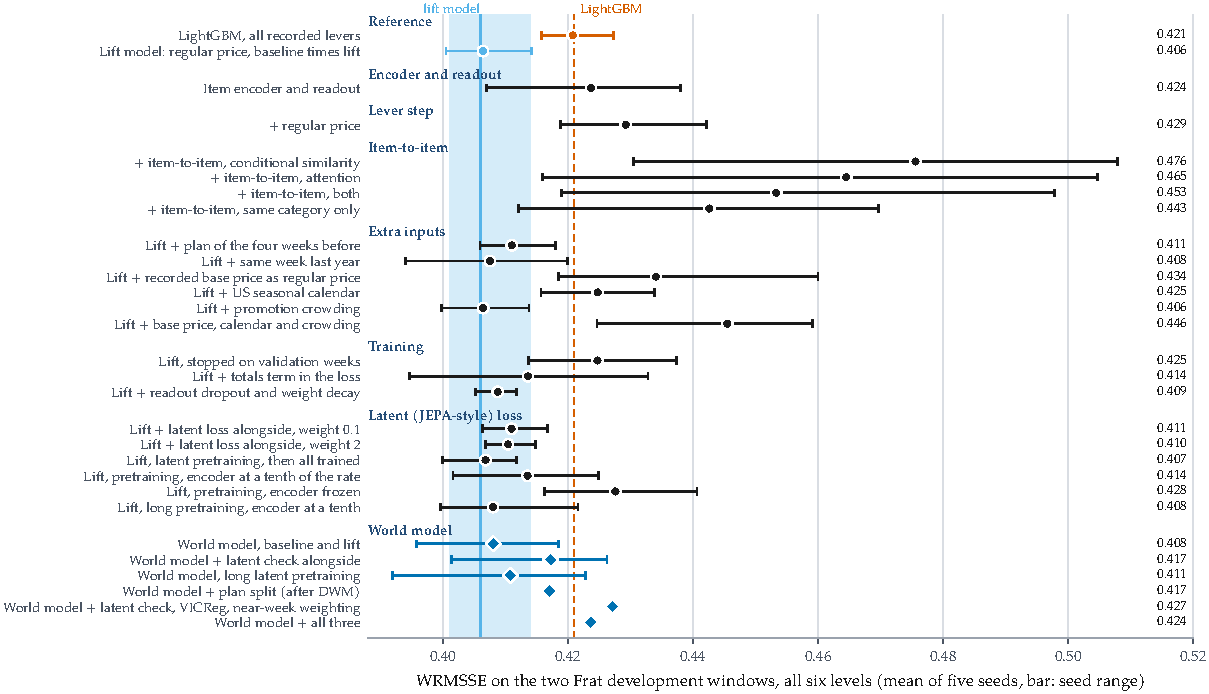
\includegraphics[width=\textwidth]{figs/fig_frat_dev.pdf}
\caption{\textbf{On Frat the gain came from building the forecast as a baseline
times a plan lift; item-to-item links, extra inputs, latent losses and the
roll-forward did not improve on it.} Each row is one configuration on the two
development windows, five seeds: mean (marker) and range (bar). Blue band: the
lift model's seed range; vertical lines: the lift model (0.406) and LightGBM
(0.421). Values below the lift model are in bold. Rows without a bar were
recorded as a mean only.}
\label{fig:fratdev}
\end{figure*}

\paragraph{What helped and what did not}
Figure~\ref{fig:fratdev} shows every configuration screened on Frat. Our item
encoder with a direct readout scored 0.424, level with LightGBM (0.421).
Building the forecast as a baseline under the nothing-planned plan times a lift
(the lift model) brought it to 0.406, better than LightGBM in all five runs and
with half the spread across seeds. Letting the 55 items in a store affect each
other, by conditional similarity, attention or both, made the forecast worse in
every version (0.443 to 0.476) and less steady; limiting it to items in the same
category narrowed the gap without closing it. Extra inputs did not help: the
plan of the four weeks before (0.411), the same week last year (0.408), the US
seasonal calendar (0.425), the count of items on promotion in the store (0.406)
and the recorded base price used as the regular price (0.434). The recorded
base price changes about twelve times a year per item and equals the shelf
price in every week without a promotion, so it is not a slow-moving regular
price.

\paragraph{Latent (JEPA-style) losses}
Following the JEPA literature~\cite{lecun2022,ijepa} and M-JEPA~\cite{mjepa}, we
added a loss that predicts the encoder's own state for the forecast weeks from
the state now and the plan, with a slowly updated copy of the encoder as the
target~\cite{byol}. No recipe beat the lift model: alongside the forecast loss
0.410 to 0.411, pretrained on the latent loss and then fine-tuned 0.407 to
0.414. With the encoder frozen after latent-only pretraining the model still
reached 0.428, so a state learned without any sales target carries most of the
forecast signal. Long pretraining followed by a slowed encoder gave the best
display-week error of any configuration (0.813 for the world model, against
0.817 for LightGBM).

\paragraph{The world model}
Rolling the state forward week by week under the plan scored 0.408, level with
the lift model on the overall score and on every lever. Three ideas from the
world-model literature, each at one untuned setting, did not help: keeping the
plan's effect apart from the no-plan state as in DWM~\cite{dwm} (0.417), a
latent check on each rolled step with a VICReg penalty~\cite{vicreg} and near
weeks weighted more as in TD-MPC2~\cite{tdmpc2} (0.427), and all three together
(0.424). Training changes did not help either: stopping at the best point on the
last 8 training weeks (0.425) took 8 of only 90 training weeks out of the
targets, and a term on summed totals in the loss (0.414) had no bias to fix,
since total forecasts were within 3\% of sales in every run. Readout dropout
with weight decay (0.409) was level and steadier, and was kept for the lift
model.

\begin{table*}[t]
\centering
\caption{\textbf{What the plan-aware models were also tested on during development: new items, combination
with LightGBM, choosing between two plans, and plans an item had rarely run.} Development windows, three
seeds (Frat combination: five). WRMSSE, lower is better, unless stated. Plan A against plan B: share of
week pairs where the forecast picks the week that sold more, and the average miss on the size of the change
(log scale).}
\label{tab:tests}
\footnotesize
\begin{tabular}{p{0.12\textwidth}p{0.50\textwidth}p{0.28\textwidth}}
\toprule
\textbf{Data} & \textbf{Model} & \textbf{Result} \\
\midrule
\multicolumn{3}{l}{\itshape New items: one product in ten never seen in training (item by store)} \\
Frat & LightGBM, new item from labels, price and plan & 1.310 \\
Frat & Lift model, borrowing from similar items & \textbf{0.890} \\
Frat & Forecast of zero & 1.510 \\
Analgesics & LightGBM, from labels, price and plan & \textbf{0.923} \\
Analgesics & Lift model, borrowing (no attribute labels) & 2.999 \\
\addlinespace[2pt]\multicolumn{3}{l}{\itshape Combination with LightGBM, weights set on a validation window (all levels)} \\
Frat & Lift model + LightGBM & \textbf{0.388} \\
Frat & World model + LightGBM & 0.390 \\
Frat & LightGBM; lift model; world model & 0.421; 0.406; 0.408 \\
Analgesics & Lift + LightGBM; world + LightGBM & 0.670; 0.668 \\
\addlinespace[2pt]\multicolumn{3}{l}{\itshape Plan A against plan B: same item and store, two weeks with different plans (Frat)} \\
Frat & LightGBM & 78.2\% right; miss 0.448 \\
Frat & Lift model & 77.4\% right; miss 0.460 \\
Frat & World model & 77.5\% right; miss 0.459 \\
Frat & World model + plan split & 77.5\% right; miss 0.458 \\
\addlinespace[2pt]\multicolumn{3}{l}{\itshape Unusual plans: a lever mix the item had in under 2\% of its weeks (item by store)} \\
Frat & LightGBM & 0.696 unusual; 0.697 usual \\
Frat & Lift model & 0.743 unusual; 0.725 usual \\
Frat & World model & 0.730 unusual; 0.730 usual \\
\bottomrule
\end{tabular}
\end{table*}


\paragraph{Beyond accuracy}
Table~\ref{tab:tests} reports four further tests. \emph{New items}: with one
product in ten held out of training, the lift model borrowing the state and
level of the ten known items in the same store with the most labels in common
scored 0.890 on the new items, against 1.310 for LightGBM fitted on labels,
price and plan, and 1.510 for a forecast of zero. On Dominick's analgesics,
where items carry no category or maker labels, borrowing failed (2.999 against
0.923): the method needs item attributes. \emph{Combination}: weighting the lift
model and LightGBM on a validation window gave the best Frat result of the study
(0.388), better than either part on display and circular weeks, because the two
make different errors in promoted weeks; on analgesics the combination was
level. Combinations were not carried to the final tests, which compare single
models. \emph{Plan A against plan B}: for pairs of weeks of the same item and
store with different plans, every model picked the week that sold more about
78\% of the time; LightGBM was marginally ahead. \emph{Unusual plans}: on lever
mixes an item had run in under 2\% of its weeks, no model degraded much and
LightGBM stayed ahead. The world model's ability to roll a plan forward did not
show as an advantage on these tests.

\subsection{Dominick's}
\label{sec:dev-dom}

\paragraph{Analgesics, the category used to set the models}
On analgesics, seasonal naive scored 1.274, the average of the last 8 weeks
0.723 and LightGBM 0.715. The lift model scored 0.676 on three seeds, and the
world model 0.667 once a totals term was removed from its loss: that term made
the total worse, pulling forecasts 9\% low (0.819 for the lift model). Training
four times longer without a stop broke the summed levels (1.473) while
item-by-store error barely moved, so a small bias in the same direction on
every item added up at the category total. Five seeds changed the picture: the
world model held (0.666) and LightGBM scored 0.702, but the lift model fell to
0.718, so a three-seed figure had flattered it.

\begin{figure*}[t]
\centering
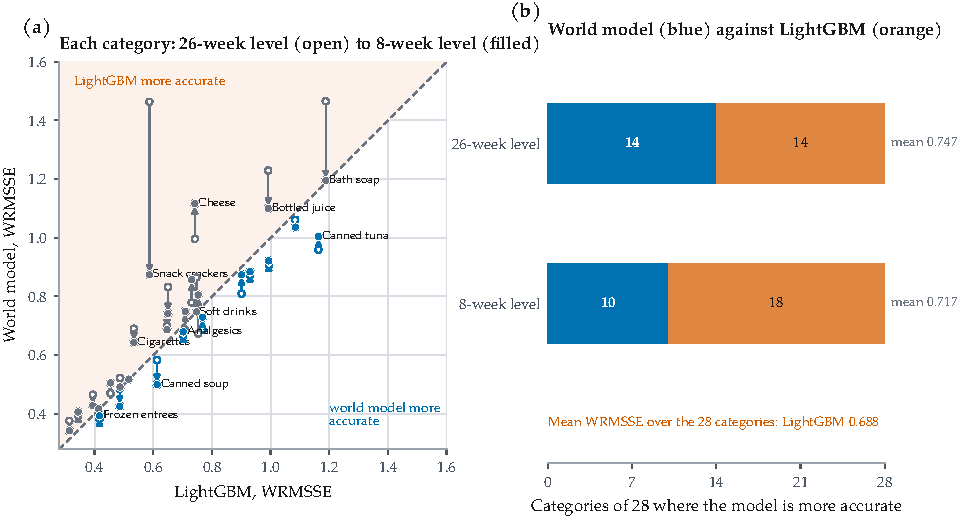
\includegraphics[width=\textwidth]{figs/fig_dom28.pdf}
\caption{\textbf{Run unchanged on all 28 Dominick's categories, the world model
set on analgesics failed badly in a few; taking each item's level from its last
8 weeks removed the worst failures but did not make it better than LightGBM on
average.} Development windows, one seed. \textbf{(a)} Each category's
WRMSSE for LightGBM (horizontal) and the world model (vertical), with the item
level from the last 26 weeks (open) and the last 8 weeks (filled); blue: the
world model is more accurate with the 8-week level. \textbf{(b)} Categories
where each model is more accurate, and the mean over the 28.}
\label{fig:dom28}
\end{figure*}

\paragraph{All 28 categories}
Run on all 28 categories with settings from analgesics, LightGBM was the most
accurate of the three in 14, the lift model in 5 and the world model in 9, with
mean WRMSSE 0.688, 0.784 and 0.747; on promoted weeks LightGBM was most accurate
in 24 of 27 (Figure~\ref{fig:dom28}, Table~\ref{tab:dom28}). Analgesics did not
generalise, which is why the paper reports every category. The failures (snack
crackers 1.463, bath soap 1.465, the lift model on soft drinks 1.406) sat at the
category total: item-by-store error was close to LightGBM's. On a six-store
sample of snack crackers the cause was in-and-out and seasonal lines: items
recorded in 8 to 20 of the last 26 weeks were 8\% of sales and the lift model
forecast them at 9 times their sales, because the model set each item's level from its 26-week
average after the item had fallen away. Capping extreme weeks did little; taking
the level from the last 8 weeks removed most of it. On all 28 categories the
8-week level brought the world model's mean to 0.717, removed the large failures
(snack crackers 1.463 to 0.874, bath soap 1.465 to 1.195) and gave a little back
in categories that had been fine, so it beat LightGBM in 10 categories against
14 before. LightGBM, which sees short recent averages directly, does not have the
problem.

\begin{table}[t]
\centering
\caption{\textbf{Across all 28 Dominick's categories LightGBM is more accurate on average; the world model
wins in 14 with its first level and 10 with the 8-week level.} Development windows, one seed (analgesics:
five), settings set on analgesics and not tuned per category. World model with the item's level from its
last 26 weeks or last 8 weeks. Lowest in each row in bold.}
\label{tab:dom28}
\footnotesize
\setlength{\tabcolsep}{4pt}
\renewcommand{\arraystretch}{1.05}
\begin{tabular}{lrrrr}
\toprule
\textbf{Category} & \textbf{LightGBM} & \textbf{Lift} & \textbf{World, 26 wk} & \textbf{World, 8 wk} \\
\midrule
Analgesics & 0.702 & 0.718 & \textbf{0.666} & 0.679 \\
Bath soap & \textbf{1.188} & 1.568 & 1.465 & 1.195 \\
Beer & \textbf{0.454} & 0.460 & 0.470 & 0.505 \\
Bottled juice & \textbf{0.992} & 1.247 & 1.229 & 1.100 \\
Canned soup & 0.613 & 0.532 & 0.583 & \textbf{0.500} \\
Canned tuna & 1.163 & 1.030 & \textbf{0.959} & 1.004 \\
Cereals & 0.753 & 0.795 & \textbf{0.673} & 0.805 \\
Cheese & \textbf{0.742} & 0.900 & 0.996 & 1.116 \\
Cigarettes & \textbf{0.534} & 0.918 & 0.690 & 0.643 \\
Cookies & \textbf{0.487} & 0.503 & 0.522 & 0.491 \\
Crackers & 0.709 & 0.967 & \textbf{0.687} & 0.749 \\
Dish detergent & \textbf{0.344} & 0.436 & 0.393 & 0.405 \\
Fabric softener & 0.414 & \textbf{0.358} & 0.397 & 0.417 \\
Front-end candies & \textbf{0.650} & 0.748 & 0.832 & 0.742 \\
Frozen dinners & 0.930 & 0.905 & \textbf{0.873} & 0.884 \\
Frozen entrees & 0.417 & \textbf{0.374} & 0.382 & 0.393 \\
Frozen juices & \textbf{0.314} & 0.360 & 0.376 & 0.342 \\
Grooming products & 0.901 & 1.208 & \textbf{0.809} & 0.874 \\
Laundry detergent & 0.768 & 0.735 & \textbf{0.687} & 0.729 \\
Oatmeal & 1.084 & \textbf{1.026} & 1.060 & 1.036 \\
Paper towels & 0.486 & 0.445 & 0.485 & \textbf{0.425} \\
Shampoos & 0.994 & 0.938 & \textbf{0.906} & 0.921 \\
Snack crackers & \textbf{0.587} & 0.959 & 1.463 & 0.874 \\
Soaps & 0.517 & 0.521 & \textbf{0.516} & 0.518 \\
Soft drinks & 0.747 & 1.406 & 0.864 & \textbf{0.747} \\
Toilet tissue & \textbf{0.394} & 0.413 & 0.465 & 0.427 \\
Toothbrushes & \textbf{0.647} & 0.671 & 0.699 & 0.686 \\
Toothpaste & \textbf{0.731} & 0.802 & 0.779 & 0.857 \\
\midrule
Mean & 0.688 & 0.784 & 0.747 & 0.717 \\
\bottomrule
\end{tabular}
\end{table}


\paragraph{Peaks and dips}
In cheese, both our model and LightGBM under-forecast promoted weeks by about a
third in the holiday window, and cheese peaks do not sit on a fixed week
relative to the holidays: they follow the chain's promotion timing, which event
flags cannot place. Figure~\ref{fig:peaks} splits forecast against sales into
promoted weeks, the weeks just after a promotion, and ordinary weeks, for six
categories. The world model did not see the dip after a promotion where the dip
is large: it forecast 1.33 times sales after a promotion in snack crackers and
1.32 in soft drinks, against 0.92 and 0.90 for LightGBM. Feeding the model's own
sales forecast into the roll-forward, so that a promotion's sales could shape the
weeks after it, fixed the soft-drink dip (1.32 to 1.00) and made the overall
score worse in four of six categories. Weighting the loss by dollar sales and by
how far a week sits from the item's usual level fixed cheese promoted weeks
(1.21 to 1.00) and was worse overall in three categories. In frozen entrees every
model, LightGBM included, forecast about 0.7 of sales after a promotion: there the
week after is stronger than any model expected.

\begin{figure*}[t]
\centering
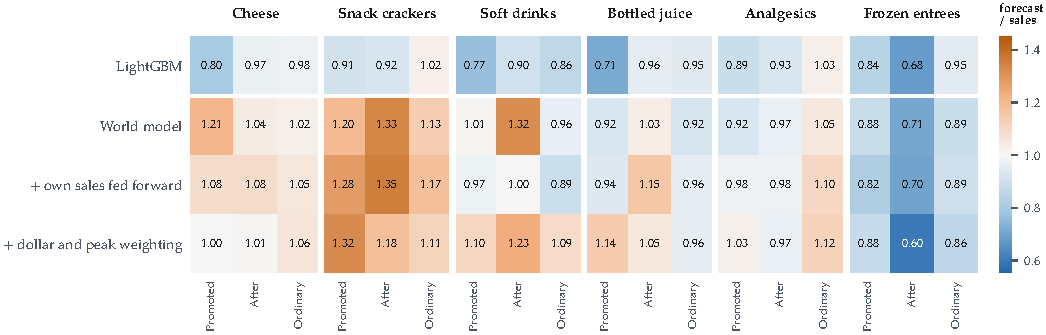
\includegraphics[width=\textwidth]{figs/fig_peaks.pdf}
\caption{\textbf{The world model over-forecast the weeks after a promotion where
shoppers had stocked up; the two fixes each repaired one category and hurt
others.} Forecast against sales (1.0 is right; orange over, blue under) in
promoted weeks, the weeks just after a promotion and ordinary weeks, Dominick's
development windows, one seed. Rows: LightGBM, the world model with the 8-week
level, with its own sales forecast fed forward, and with the loss weighted by
dollar sales and by peaks.}
\label{fig:peaks}
\end{figure*}

\paragraph{From the first world model to the one tested}
Figure~\ref{fig:ladder} follows the world model on the six categories through
the changes kept, three seeds each. Across seeds the first version was unsteady:
its range within a category was 0.04 to 0.38, against under 0.03 for LightGBM,
and on the mean LightGBM was ahead in five of six. Brand switching fixed what it
was built for: in snack crackers and soft drinks, where promoted weeks broke the
total, it was better on every seed (0.813 to 0.752, 0.902 to 0.789) and
item-by-store error improved too. The fitted share of the summed lift that the category total keeps
(Figure~\ref{fig:ladder}g) is 0.00 to 0.66 in snack crackers, against about 0.9
in bottled juice, analgesics and frozen entrees: in snack crackers the summed
item lifts overstated the category total, and the fit took most of it back.
Where it comes out at 1.0 the step changes nothing, a built-in check. The
direction agrees with van Heerde, Gupta and Wittink's household
estimates~\cite{vanheerde2003}, but the share is fitted to make totals right; it
is not an estimate of switching. Normalising the rolled state narrowed the seed range in five of six
categories, and averaging three fits per run with normalisation gave the
steadiest version (range 0.05 or less in five categories) and the candidate for
the final test: better than LightGBM on the three-seed mean in analgesics (0.622
against 0.701), frozen entrees (0.391 against 0.419) and soft drinks (0.743
against 0.759). One snack-cracker run of the three failed (1.806): its second
window's category total broke with promoted weeks forecast at 2.6 times sales
while item-by-store error stayed normal, so the summed promotion lift can still
run away on one fit in three. Twice the training steps, screened after the final
tests were fixed, was better in two categories, worse in two, level in one and
mixed in one, and was not kept.

\begin{figure*}[t]
\centering
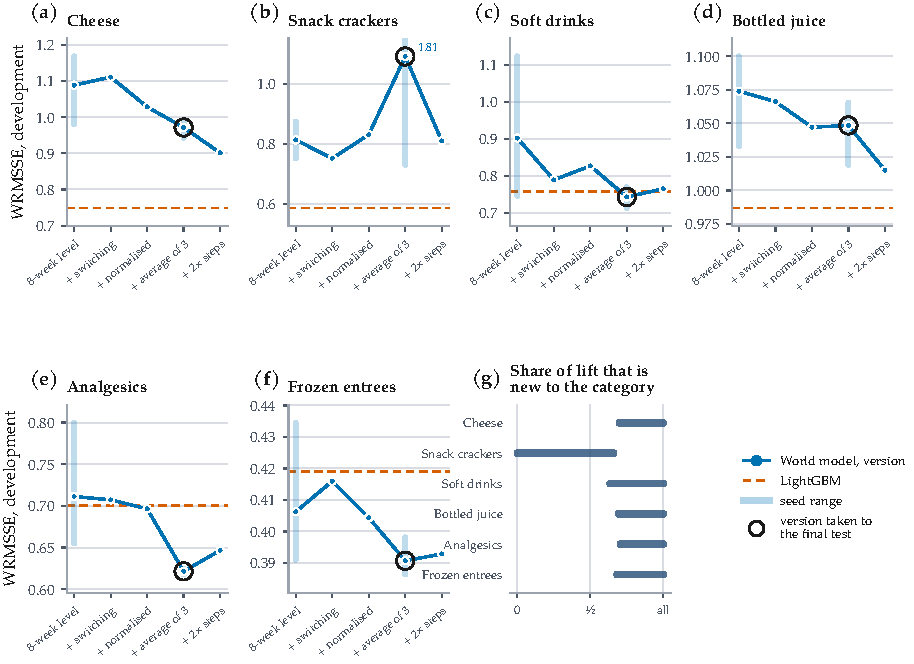
\includegraphics[width=\textwidth]{figs/fig_ladder.pdf}
\caption{\textbf{Brand switching, a normalised roll-forward and averaging three
fits took the world model past LightGBM in three of six categories on the
development windows, and the switching step learned how much of a promotion's
lift is new to the category.} \textbf{(a--f)} Development WRMSSE of each version,
three-seed means; shaded bars: seed range of the first version and of the one
taken to the final test (circled); dashed: LightGBM. \textbf{(g)} The fitted share of the summed promotion lift that the category
total keeps, the split that makes category totals fit best (not an estimate of
switching), range over runs.}
\label{fig:ladder}
\end{figure*}

\paragraph{Other changes}
Showing the model both its 26-week and its recent levels as inputs, instead of
setting its scale by the recent level, was the best world-model version in four
of ten categories but did not fix snack crackers (1.515) or soft drinks (1.069):
the model did not learn to switch to the recent level when the long level still
set its scale. Item role labels (new line, in-and-out, volume driver, long tail,
high-low, promotion-responsive, core), assigned from each item's own sales before
the windows, moved LightGBM by at most 0.013, since it reads the same information
from its history, and moved the world model in both directions; letting the role
pick the level broke snack crackers (2.422). We did not call the volume drivers
key value items, since a key-value-item list rests on shopper price perception,
which these data do not record.

\subsection{M5}
\label{sec:dev-m5}

\begin{table}[t]
\centering
\caption{\textbf{On the M5 practice window, only the normalised roll-forward separated the world model from
LightGBM; no later change beat it.} WRMSSE over all 12 levels, 25 April to 22 May 2016. A screened change
was kept only if it lowered the score, and a change that doubles the cost only if by more than the seed
range (0.029).}
\label{tab:m5dev}
\footnotesize
\begin{tabular}{p{0.58\columnwidth}rr}
\toprule
\textbf{Model or change} & \textbf{Mean} & \textbf{Seed range} \\
\midrule
Seasonal naive & 0.870 &  \\
LightGBM, one model per store & 0.715 &  \\
Lift model (3 seeds) & 0.713 & 0.683 to 0.734 \\
Item encoder and readout (5 seeds) & 0.699 & 0.669 to 0.724 \\
World model (3 seeds) & 0.707 & 0.679 to 0.750 \\
World model + normalised roll-forward (3 seeds) & 0.656 & 0.646 to 0.675 \\
+ average of three fits (1 run) & 0.665 &  \\
+ weekday as seven inputs (seed 1) & 0.653 &  \\
+ weekday and event kinds (seed 1) & 0.646 &  \\
+ 60,000 training steps (seed 1) & 0.642 &  \\
+ item level against past-year level (seed 1) & 0.680 &  \\
\bottomrule
\end{tabular}
\end{table}


On the M5 practice window (Table~\ref{tab:m5dev}), the item encoder with a
direct readout scored 0.699 over five seeds against 0.715 for LightGBM, and the
lift and world models were level with LightGBM over three seeds (0.713 and
0.707). Normalising the rolled state was the one change that separated the world
model: 0.656, with its worst seed (0.675) better than the best seed without it
(0.680), all of the gain at the totals and the seed range cut from 0.070 to
0.029. It helped on M5's 28 daily steps and not on Dominick's 8 weekly steps,
which fits the reading that it stops the state drifting over a long roll.
Averaging three fits did not help on M5 (0.665), where single fits were already
steady.

After the official test month, an error analysis of the world model found its
2.6\% excess in Foods (+3.9\%), in one store (CA\_3, +7.5\%), and on Sundays and
Mondays (+5.1\%, +6.4\%), not growing with the horizon. Grouped by sales in the
28 days before the test, the excess came from items that had been selling fast
(+5.4\% and +6.1\% on items selling 3 to 10 and over 10 a day). Four changes
were screened on the practice window under rules written before screening:
weekday as seven inputs, event kinds, twice the training steps, and the item's
level against its past-year level. None beat the original
(Table~\ref{tab:m5dev}), so there was no second version. On the practice window
every version under-forecast by 4\% to 6\%, while on the test month the world
model over-forecast by 2.6\%: the sign of the level error changed between
adjacent months, so a fix tuned on one would not carry to the next. That
finding is what led to the confirmation months of \S\ref{sec:onemonth}.

% =====================================================================

